\documentclass[]{article}
\usepackage{lmodern}
\usepackage{amssymb,amsmath}
\usepackage{ifxetex,ifluatex}
\usepackage{fixltx2e} % provides \textsubscript
\ifnum 0\ifxetex 1\fi\ifluatex 1\fi=0 % if pdftex
  \usepackage[T1]{fontenc}
  \usepackage[utf8]{inputenc}
\else % if luatex or xelatex
  \ifxetex
    \usepackage{mathspec}
  \else
    \usepackage{fontspec}
  \fi
  \defaultfontfeatures{Ligatures=TeX,Scale=MatchLowercase}
\fi
% use upquote if available, for straight quotes in verbatim environments
\IfFileExists{upquote.sty}{\usepackage{upquote}}{}
% use microtype if available
\IfFileExists{microtype.sty}{%
\usepackage{microtype}
\UseMicrotypeSet[protrusion]{basicmath} % disable protrusion for tt fonts
}{}
\usepackage[margin=1in]{geometry}
\usepackage{hyperref}
\hypersetup{unicode=true,
            pdftitle={Statistical analysis},
            pdfborder={0 0 0},
            breaklinks=true}
\urlstyle{same}  % don't use monospace font for urls
\usepackage{longtable,booktabs}
\usepackage{graphicx,grffile}
\makeatletter
\def\maxwidth{\ifdim\Gin@nat@width>\linewidth\linewidth\else\Gin@nat@width\fi}
\def\maxheight{\ifdim\Gin@nat@height>\textheight\textheight\else\Gin@nat@height\fi}
\makeatother
% Scale images if necessary, so that they will not overflow the page
% margins by default, and it is still possible to overwrite the defaults
% using explicit options in \includegraphics[width, height, ...]{}
\setkeys{Gin}{width=\maxwidth,height=\maxheight,keepaspectratio}
\IfFileExists{parskip.sty}{%
\usepackage{parskip}
}{% else
\setlength{\parindent}{0pt}
\setlength{\parskip}{6pt plus 2pt minus 1pt}
}
\setlength{\emergencystretch}{3em}  % prevent overfull lines
\providecommand{\tightlist}{%
  \setlength{\itemsep}{0pt}\setlength{\parskip}{0pt}}
\setcounter{secnumdepth}{5}
% Redefines (sub)paragraphs to behave more like sections
\ifx\paragraph\undefined\else
\let\oldparagraph\paragraph
\renewcommand{\paragraph}[1]{\oldparagraph{#1}\mbox{}}
\fi
\ifx\subparagraph\undefined\else
\let\oldsubparagraph\subparagraph
\renewcommand{\subparagraph}[1]{\oldsubparagraph{#1}\mbox{}}
\fi

%%% Use protect on footnotes to avoid problems with footnotes in titles
\let\rmarkdownfootnote\footnote%
\def\footnote{\protect\rmarkdownfootnote}

%%% Change title format to be more compact
\usepackage{titling}

% Create subtitle command for use in maketitle
\newcommand{\subtitle}[1]{
  \posttitle{
    \begin{center}\large#1\end{center}
    }
}

\setlength{\droptitle}{-2em}
  \title{Statistical analysis}
  \pretitle{\vspace{\droptitle}\centering\huge}
  \posttitle{\par}
  \author{}
  \preauthor{}\postauthor{}
  \date{}
  \predate{}\postdate{}


\begin{document}
\maketitle

\section{Project Summary}\label{project-summary}

\textbf{Collaborators}

J.T. Lennon, \emph{Indiana University, Bloomington, IN}

S.W. Wilhelm, \emph{University of Tennessee - Knoxville, Knoxville TN}

\textbf{Project questions}

\begin{enumerate}
\def\labelenumi{\arabic{enumi}.}
\tightlist
\item
  Does resource stoichiometry affect the growth rate of
  \emph{Synechococcus}?
\item
  How does resource stoichiometry alter ecological dynamics?
\item
  Does stoichiometry alter phenotypic (co)evolution in cyanobacteria and
  phage?
\end{enumerate}

\textbf{Data collection}

Briefly, all data for this project was collected during a long term
continuous culture experimental evolution study with
\emph{Synechococcus} and SRIM-8 cyanomyophage.

For a complete description of the materials and methods for this
repository, see Larsen \emph{et al.} 2016.

Funding for this project was provided in part by the National Science
Foundation, Michigan State University BEACON Center for Evolution in
Action, and Indiana University.

\newpage

\tableofcontents
\newpage

\section{\texorpdfstring{Physiological growth: Does nutrient
stoichiometry affect the growth rate of
\emph{Synechococcus}?}{Physiological growth: Does nutrient stoichiometry affect the growth rate of Synechococcus?}}\label{physiological-growth-does-nutrient-stoichiometry-affect-the-growth-rate-of-synechococcus}

\textbf{Overview}: In this experiment, we tested for growth enhancement
with the addtion of nitrogen (N), phosphosphorus (P), or the addition of
both nutrients to our stoichiometrically modified AN media (Lennon
\emph{et al.} 2007; see Larsen \emph{et al.} 2016 Table S1). Population
growth curve data was collected on a Biotek Synergy Mx instrument loaded
with software version 2.01.12.

\subsection{Summary of Major Results}\label{summary-of-major-results}

\begin{enumerate}
\def\labelenumi{\arabic{enumi}.}
\tightlist
\item
  Addition of N or P to the N-limited or P-limited base medium,
  respectively, increased \emph{Synechococcus} maximum growth rate
  (Figure 1) and percent change in growth (Figure 2) in batch culture as
  compared to control cultures without the addition of N or P.
\end{enumerate}

\newpage

\subsection{\texorpdfstring{\emph{Synechococcus} growth rates with
response to nutrient
addition}{Synechococcus growth rates with response to nutrient addition}}\label{synechococcus-growth-rates-with-response-to-nutrient-addition}

\begin{figure}[htbp]
\centering
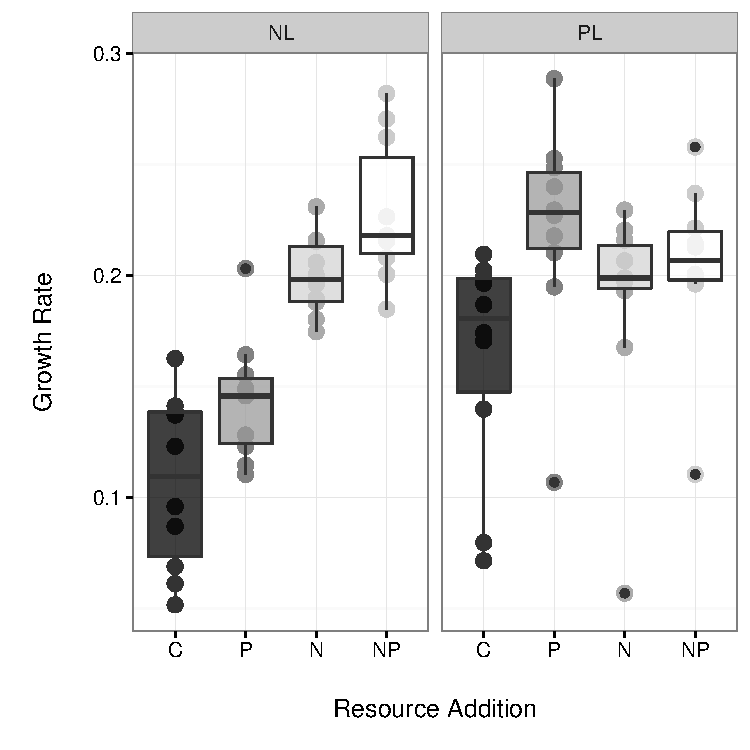
\includegraphics{analysis_ecoevostoich_files/figure-latex/gr-vis-1.pdf}
\caption{Nitrogen (N), phosphorus (P), or NP addition to the base
N-limited and P-limited media used in the chemostat experiment. Culture
controls (C) did not contain additional N or P.}
\end{figure}

\newpage

\subsubsection{Growth rate ANOVA tables}\label{growth-rate-anova-tables}

\textbf{N-limited}

\begin{longtable}[]{@{}cccccc@{}}
\caption{ANOVA table for NL nutrient addition}\tabularnewline
\toprule
\begin{minipage}[b]{0.19\columnwidth}\centering\strut
~\strut
\end{minipage} & \begin{minipage}[b]{0.06\columnwidth}\centering\strut
Df\strut
\end{minipage} & \begin{minipage}[b]{0.10\columnwidth}\centering\strut
Sum Sq\strut
\end{minipage} & \begin{minipage}[b]{0.12\columnwidth}\centering\strut
Mean Sq\strut
\end{minipage} & \begin{minipage}[b]{0.12\columnwidth}\centering\strut
F value\strut
\end{minipage} & \begin{minipage}[b]{0.12\columnwidth}\centering\strut
Pr(\textgreater{}F)\strut
\end{minipage}\tabularnewline
\midrule
\endfirsthead
\toprule
\begin{minipage}[b]{0.19\columnwidth}\centering\strut
~\strut
\end{minipage} & \begin{minipage}[b]{0.06\columnwidth}\centering\strut
Df\strut
\end{minipage} & \begin{minipage}[b]{0.10\columnwidth}\centering\strut
Sum Sq\strut
\end{minipage} & \begin{minipage}[b]{0.12\columnwidth}\centering\strut
Mean Sq\strut
\end{minipage} & \begin{minipage}[b]{0.12\columnwidth}\centering\strut
F value\strut
\end{minipage} & \begin{minipage}[b]{0.12\columnwidth}\centering\strut
Pr(\textgreater{}F)\strut
\end{minipage}\tabularnewline
\midrule
\endhead
\begin{minipage}[t]{0.19\columnwidth}\centering\strut
\textbf{med.add}\strut
\end{minipage} & \begin{minipage}[t]{0.06\columnwidth}\centering\strut
3\strut
\end{minipage} & \begin{minipage}[t]{0.10\columnwidth}\centering\strut
0.08993\strut
\end{minipage} & \begin{minipage}[t]{0.12\columnwidth}\centering\strut
0.02998\strut
\end{minipage} & \begin{minipage}[t]{0.12\columnwidth}\centering\strut
33.3\strut
\end{minipage} & \begin{minipage}[t]{0.12\columnwidth}\centering\strut
1.743e-10\strut
\end{minipage}\tabularnewline
\begin{minipage}[t]{0.19\columnwidth}\centering\strut
\textbf{Residuals}\strut
\end{minipage} & \begin{minipage}[t]{0.06\columnwidth}\centering\strut
36\strut
\end{minipage} & \begin{minipage}[t]{0.10\columnwidth}\centering\strut
0.0324\strut
\end{minipage} & \begin{minipage}[t]{0.12\columnwidth}\centering\strut
0.0009001\strut
\end{minipage} & \begin{minipage}[t]{0.12\columnwidth}\centering\strut
NA\strut
\end{minipage} & \begin{minipage}[t]{0.12\columnwidth}\centering\strut
NA\strut
\end{minipage}\tabularnewline
\bottomrule
\end{longtable}

\begin{longtable}[]{@{}ccccc@{}}
\caption{Posthoc comparisons using Tukey HSD}\tabularnewline
\toprule
\begin{minipage}[b]{0.13\columnwidth}\centering\strut
~\strut
\end{minipage} & \begin{minipage}[b]{0.16\columnwidth}\centering\strut
diff\strut
\end{minipage} & \begin{minipage}[b]{0.16\columnwidth}\centering\strut
lwr\strut
\end{minipage} & \begin{minipage}[b]{0.16\columnwidth}\centering\strut
upr\strut
\end{minipage} & \begin{minipage}[b]{0.16\columnwidth}\centering\strut
p adj\strut
\end{minipage}\tabularnewline
\midrule
\endfirsthead
\toprule
\begin{minipage}[b]{0.13\columnwidth}\centering\strut
~\strut
\end{minipage} & \begin{minipage}[b]{0.16\columnwidth}\centering\strut
diff\strut
\end{minipage} & \begin{minipage}[b]{0.16\columnwidth}\centering\strut
lwr\strut
\end{minipage} & \begin{minipage}[b]{0.16\columnwidth}\centering\strut
upr\strut
\end{minipage} & \begin{minipage}[b]{0.16\columnwidth}\centering\strut
p adj\strut
\end{minipage}\tabularnewline
\midrule
\endhead
\begin{minipage}[t]{0.13\columnwidth}\centering\strut
\textbf{N-C}\strut
\end{minipage} & \begin{minipage}[t]{0.16\columnwidth}\centering\strut
\textbf{0.0929}\strut
\end{minipage} & \begin{minipage}[t]{0.16\columnwidth}\centering\strut
\textbf{0.05677}\strut
\end{minipage} & \begin{minipage}[t]{0.16\columnwidth}\centering\strut
\textbf{0.129}\strut
\end{minipage} & \begin{minipage}[t]{0.16\columnwidth}\centering\strut
\textbf{2.426e-07}\strut
\end{minipage}\tabularnewline
\begin{minipage}[t]{0.13\columnwidth}\centering\strut
\textbf{NP-C}\strut
\end{minipage} & \begin{minipage}[t]{0.16\columnwidth}\centering\strut
\textbf{0.1218}\strut
\end{minipage} & \begin{minipage}[t]{0.16\columnwidth}\centering\strut
\textbf{0.0857}\strut
\end{minipage} & \begin{minipage}[t]{0.16\columnwidth}\centering\strut
\textbf{0.158}\strut
\end{minipage} & \begin{minipage}[t]{0.16\columnwidth}\centering\strut
\textbf{4.542e-10}\strut
\end{minipage}\tabularnewline
\begin{minipage}[t]{0.13\columnwidth}\centering\strut
\textbf{P-C}\strut
\end{minipage} & \begin{minipage}[t]{0.16\columnwidth}\centering\strut
\textbf{0.03716}\strut
\end{minipage} & \begin{minipage}[t]{0.16\columnwidth}\centering\strut
\textbf{0.001027}\strut
\end{minipage} & \begin{minipage}[t]{0.16\columnwidth}\centering\strut
\textbf{0.0733}\strut
\end{minipage} & \begin{minipage}[t]{0.16\columnwidth}\centering\strut
\textbf{0.04188}\strut
\end{minipage}\tabularnewline
\begin{minipage}[t]{0.13\columnwidth}\centering\strut
\textbf{NP-N}\strut
\end{minipage} & \begin{minipage}[t]{0.16\columnwidth}\centering\strut
0.02893\strut
\end{minipage} & \begin{minipage}[t]{0.16\columnwidth}\centering\strut
-0.007204\strut
\end{minipage} & \begin{minipage}[t]{0.16\columnwidth}\centering\strut
0.06507\strut
\end{minipage} & \begin{minipage}[t]{0.16\columnwidth}\centering\strut
0.1551\strut
\end{minipage}\tabularnewline
\begin{minipage}[t]{0.13\columnwidth}\centering\strut
\textbf{P-N}\strut
\end{minipage} & \begin{minipage}[t]{0.16\columnwidth}\centering\strut
\textbf{-0.05574}\strut
\end{minipage} & \begin{minipage}[t]{0.16\columnwidth}\centering\strut
\textbf{-0.09188}\strut
\end{minipage} & \begin{minipage}[t]{0.16\columnwidth}\centering\strut
\textbf{-0.01961}\strut
\end{minipage} & \begin{minipage}[t]{0.16\columnwidth}\centering\strut
\textbf{0.001056}\strut
\end{minipage}\tabularnewline
\begin{minipage}[t]{0.13\columnwidth}\centering\strut
\textbf{P-NP}\strut
\end{minipage} & \begin{minipage}[t]{0.16\columnwidth}\centering\strut
\textbf{-0.08467}\strut
\end{minipage} & \begin{minipage}[t]{0.16\columnwidth}\centering\strut
\textbf{-0.1208}\strut
\end{minipage} & \begin{minipage}[t]{0.16\columnwidth}\centering\strut
\textbf{-0.04854}\strut
\end{minipage} & \begin{minipage}[t]{0.16\columnwidth}\centering\strut
\textbf{1.564e-06}\strut
\end{minipage}\tabularnewline
\bottomrule
\end{longtable}

\textbf{P-limited}

\begin{longtable}[]{@{}cccccc@{}}
\caption{ANOVA table for PL nutrient addition}\tabularnewline
\toprule
\begin{minipage}[b]{0.19\columnwidth}\centering\strut
~\strut
\end{minipage} & \begin{minipage}[b]{0.06\columnwidth}\centering\strut
Df\strut
\end{minipage} & \begin{minipage}[b]{0.10\columnwidth}\centering\strut
Sum Sq\strut
\end{minipage} & \begin{minipage}[b]{0.12\columnwidth}\centering\strut
Mean Sq\strut
\end{minipage} & \begin{minipage}[b]{0.12\columnwidth}\centering\strut
F value\strut
\end{minipage} & \begin{minipage}[b]{0.12\columnwidth}\centering\strut
Pr(\textgreater{}F)\strut
\end{minipage}\tabularnewline
\midrule
\endfirsthead
\toprule
\begin{minipage}[b]{0.19\columnwidth}\centering\strut
~\strut
\end{minipage} & \begin{minipage}[b]{0.06\columnwidth}\centering\strut
Df\strut
\end{minipage} & \begin{minipage}[b]{0.10\columnwidth}\centering\strut
Sum Sq\strut
\end{minipage} & \begin{minipage}[b]{0.12\columnwidth}\centering\strut
Mean Sq\strut
\end{minipage} & \begin{minipage}[b]{0.12\columnwidth}\centering\strut
F value\strut
\end{minipage} & \begin{minipage}[b]{0.12\columnwidth}\centering\strut
Pr(\textgreater{}F)\strut
\end{minipage}\tabularnewline
\midrule
\endhead
\begin{minipage}[t]{0.19\columnwidth}\centering\strut
\textbf{med.add}\strut
\end{minipage} & \begin{minipage}[t]{0.06\columnwidth}\centering\strut
3\strut
\end{minipage} & \begin{minipage}[t]{0.10\columnwidth}\centering\strut
0.01865\strut
\end{minipage} & \begin{minipage}[t]{0.12\columnwidth}\centering\strut
0.006215\strut
\end{minipage} & \begin{minipage}[t]{0.12\columnwidth}\centering\strut
2.845\strut
\end{minipage} & \begin{minipage}[t]{0.12\columnwidth}\centering\strut
0.05117\strut
\end{minipage}\tabularnewline
\begin{minipage}[t]{0.19\columnwidth}\centering\strut
\textbf{Residuals}\strut
\end{minipage} & \begin{minipage}[t]{0.06\columnwidth}\centering\strut
36\strut
\end{minipage} & \begin{minipage}[t]{0.10\columnwidth}\centering\strut
0.07864\strut
\end{minipage} & \begin{minipage}[t]{0.12\columnwidth}\centering\strut
0.002184\strut
\end{minipage} & \begin{minipage}[t]{0.12\columnwidth}\centering\strut
NA\strut
\end{minipage} & \begin{minipage}[t]{0.12\columnwidth}\centering\strut
NA\strut
\end{minipage}\tabularnewline
\bottomrule
\end{longtable}

\begin{longtable}[]{@{}ccccc@{}}
\caption{Posthoc comparisons using Tukey HSD}\tabularnewline
\toprule
\begin{minipage}[b]{0.13\columnwidth}\centering\strut
~\strut
\end{minipage} & \begin{minipage}[b]{0.14\columnwidth}\centering\strut
diff\strut
\end{minipage} & \begin{minipage}[b]{0.16\columnwidth}\centering\strut
lwr\strut
\end{minipage} & \begin{minipage}[b]{0.13\columnwidth}\centering\strut
upr\strut
\end{minipage} & \begin{minipage}[b]{0.13\columnwidth}\centering\strut
p adj\strut
\end{minipage}\tabularnewline
\midrule
\endfirsthead
\toprule
\begin{minipage}[b]{0.13\columnwidth}\centering\strut
~\strut
\end{minipage} & \begin{minipage}[b]{0.14\columnwidth}\centering\strut
diff\strut
\end{minipage} & \begin{minipage}[b]{0.16\columnwidth}\centering\strut
lwr\strut
\end{minipage} & \begin{minipage}[b]{0.13\columnwidth}\centering\strut
upr\strut
\end{minipage} & \begin{minipage}[b]{0.13\columnwidth}\centering\strut
p adj\strut
\end{minipage}\tabularnewline
\midrule
\endhead
\begin{minipage}[t]{0.13\columnwidth}\centering\strut
\textbf{N-C}\strut
\end{minipage} & \begin{minipage}[t]{0.14\columnwidth}\centering\strut
0.02548\strut
\end{minipage} & \begin{minipage}[t]{0.16\columnwidth}\centering\strut
-0.03081\strut
\end{minipage} & \begin{minipage}[t]{0.13\columnwidth}\centering\strut
0.08178\strut
\end{minipage} & \begin{minipage}[t]{0.13\columnwidth}\centering\strut
0.619\strut
\end{minipage}\tabularnewline
\begin{minipage}[t]{0.13\columnwidth}\centering\strut
\textbf{NP-C}\strut
\end{minipage} & \begin{minipage}[t]{0.14\columnwidth}\centering\strut
0.04166\strut
\end{minipage} & \begin{minipage}[t]{0.16\columnwidth}\centering\strut
-0.01463\strut
\end{minipage} & \begin{minipage}[t]{0.13\columnwidth}\centering\strut
0.09796\strut
\end{minipage} & \begin{minipage}[t]{0.13\columnwidth}\centering\strut
0.2094\strut
\end{minipage}\tabularnewline
\begin{minipage}[t]{0.13\columnwidth}\centering\strut
\textbf{P-C}\strut
\end{minipage} & \begin{minipage}[t]{0.14\columnwidth}\centering\strut
\textbf{0.05857}\strut
\end{minipage} & \begin{minipage}[t]{0.16\columnwidth}\centering\strut
\textbf{0.002277}\strut
\end{minipage} & \begin{minipage}[t]{0.13\columnwidth}\centering\strut
\textbf{0.1149}\strut
\end{minipage} & \begin{minipage}[t]{0.13\columnwidth}\centering\strut
\textbf{0.03881}\strut
\end{minipage}\tabularnewline
\begin{minipage}[t]{0.13\columnwidth}\centering\strut
\textbf{NP-N}\strut
\end{minipage} & \begin{minipage}[t]{0.14\columnwidth}\centering\strut
0.01618\strut
\end{minipage} & \begin{minipage}[t]{0.16\columnwidth}\centering\strut
-0.04011\strut
\end{minipage} & \begin{minipage}[t]{0.13\columnwidth}\centering\strut
0.07247\strut
\end{minipage} & \begin{minipage}[t]{0.13\columnwidth}\centering\strut
0.8656\strut
\end{minipage}\tabularnewline
\begin{minipage}[t]{0.13\columnwidth}\centering\strut
\textbf{P-N}\strut
\end{minipage} & \begin{minipage}[t]{0.14\columnwidth}\centering\strut
0.03309\strut
\end{minipage} & \begin{minipage}[t]{0.16\columnwidth}\centering\strut
-0.02321\strut
\end{minipage} & \begin{minipage}[t]{0.13\columnwidth}\centering\strut
0.08938\strut
\end{minipage} & \begin{minipage}[t]{0.13\columnwidth}\centering\strut
0.4008\strut
\end{minipage}\tabularnewline
\begin{minipage}[t]{0.13\columnwidth}\centering\strut
\textbf{P-NP}\strut
\end{minipage} & \begin{minipage}[t]{0.14\columnwidth}\centering\strut
0.01691\strut
\end{minipage} & \begin{minipage}[t]{0.16\columnwidth}\centering\strut
-0.03939\strut
\end{minipage} & \begin{minipage}[t]{0.13\columnwidth}\centering\strut
0.0732\strut
\end{minipage} & \begin{minipage}[t]{0.13\columnwidth}\centering\strut
0.8498\strut
\end{minipage}\tabularnewline
\bottomrule
\end{longtable}

\newpage

\subsection{Percent Change in Growth}\label{percent-change-in-growth}

\begin{figure}[htbp]
\centering
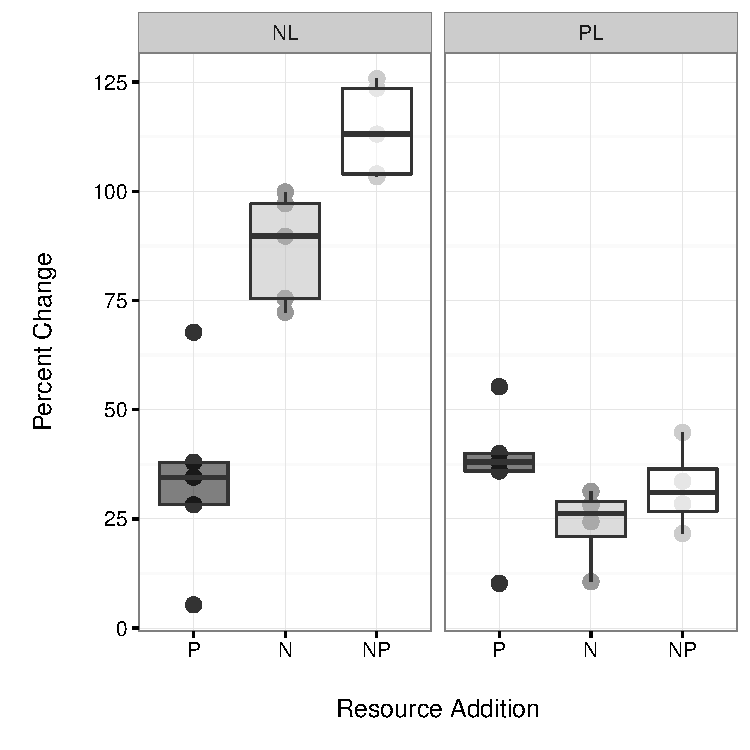
\includegraphics{analysis_ecoevostoich_files/figure-latex/perc.change-1.pdf}
\caption{Percent change in growth rate between control and nutrient
additions(N, P, or NP) cultures. NL = N-limited; PL = P-limited}
\end{figure}

\newpage

\subsubsection{Growth rate t-test
tables}\label{growth-rate-t-test-tables}

\textbf{N-limited}

\begin{longtable}[]{@{}cccc@{}}
\caption{t-test table for NL nutrient addition}\tabularnewline
\toprule
\begin{minipage}[b]{0.21\columnwidth}\centering\strut
Test statistic\strut
\end{minipage} & \begin{minipage}[b]{0.07\columnwidth}\centering\strut
df\strut
\end{minipage} & \begin{minipage}[b]{0.16\columnwidth}\centering\strut
P value\strut
\end{minipage} & \begin{minipage}[b]{0.30\columnwidth}\centering\strut
Alternative hypothesis\strut
\end{minipage}\tabularnewline
\midrule
\endfirsthead
\toprule
\begin{minipage}[b]{0.21\columnwidth}\centering\strut
Test statistic\strut
\end{minipage} & \begin{minipage}[b]{0.07\columnwidth}\centering\strut
df\strut
\end{minipage} & \begin{minipage}[b]{0.16\columnwidth}\centering\strut
P value\strut
\end{minipage} & \begin{minipage}[b]{0.30\columnwidth}\centering\strut
Alternative hypothesis\strut
\end{minipage}\tabularnewline
\midrule
\endhead
\begin{minipage}[t]{0.21\columnwidth}\centering\strut
4.546\strut
\end{minipage} & \begin{minipage}[t]{0.07\columnwidth}\centering\strut
6.271\strut
\end{minipage} & \begin{minipage}[t]{0.16\columnwidth}\centering\strut
0.001749 * *\strut
\end{minipage} & \begin{minipage}[t]{0.30\columnwidth}\centering\strut
greater\strut
\end{minipage}\tabularnewline
\bottomrule
\end{longtable}

\textbf{P-limited}

\begin{longtable}[]{@{}cccc@{}}
\caption{t-test table for PL nutrient addition}\tabularnewline
\toprule
\begin{minipage}[b]{0.21\columnwidth}\centering\strut
Test statistic\strut
\end{minipage} & \begin{minipage}[b]{0.07\columnwidth}\centering\strut
df\strut
\end{minipage} & \begin{minipage}[b]{0.12\columnwidth}\centering\strut
P value\strut
\end{minipage} & \begin{minipage}[b]{0.30\columnwidth}\centering\strut
Alternative hypothesis\strut
\end{minipage}\tabularnewline
\midrule
\endfirsthead
\toprule
\begin{minipage}[b]{0.21\columnwidth}\centering\strut
Test statistic\strut
\end{minipage} & \begin{minipage}[b]{0.07\columnwidth}\centering\strut
df\strut
\end{minipage} & \begin{minipage}[b]{0.12\columnwidth}\centering\strut
P value\strut
\end{minipage} & \begin{minipage}[b]{0.30\columnwidth}\centering\strut
Alternative hypothesis\strut
\end{minipage}\tabularnewline
\midrule
\endhead
\begin{minipage}[t]{0.21\columnwidth}\centering\strut
1.432\strut
\end{minipage} & \begin{minipage}[t]{0.07\columnwidth}\centering\strut
6.442\strut
\end{minipage} & \begin{minipage}[t]{0.12\columnwidth}\centering\strut
0.09939\strut
\end{minipage} & \begin{minipage}[t]{0.30\columnwidth}\centering\strut
greater\strut
\end{minipage}\tabularnewline
\bottomrule
\end{longtable}

\newpage

\section{Population Dynamics: Does nutrient stoichiometry affect
temporal population
dynamics?}\label{population-dynamics-does-nutrient-stoichiometry-affect-temporal-population-dynamics}

\textbf{Overview}: In this experiment, whole samples were collected from
each chemostat system three times per week for \textasciitilde{}5
months. Each sample was processed, stained, and counted using
epi-fluorescence on a Zeiss microscope and quantified using Axiovision
software. Statistics for these data include repeated measures anova
(RMANOVA), stability (1/Coefficient of Variation), and cross-correlation
analyses on whitened data using SAS.

\subsection{Summary of Major Results}\label{summary-of-major-results-1}

\begin{enumerate}
\def\labelenumi{\arabic{enumi}.}
\tightlist
\item
  Stoichiometry significantly affected \emph{Synechococcus} and phage
  densities. RMANOVA
\item
  Altered mean and stability of the populations
\item
  Modified the temporal coherence, or synchrony, of the
  \emph{Synechococcus}-phage dynamics, suggesting ecological
  ramifications of stoichiometry.
\end{enumerate}

\newpage

\subsection{Chemostat-level
comparisons}\label{chemostat-level-comparisons}

\subsubsection{Population dynamics}\label{population-dynamics}

\begin{figure}[htbp]
\centering
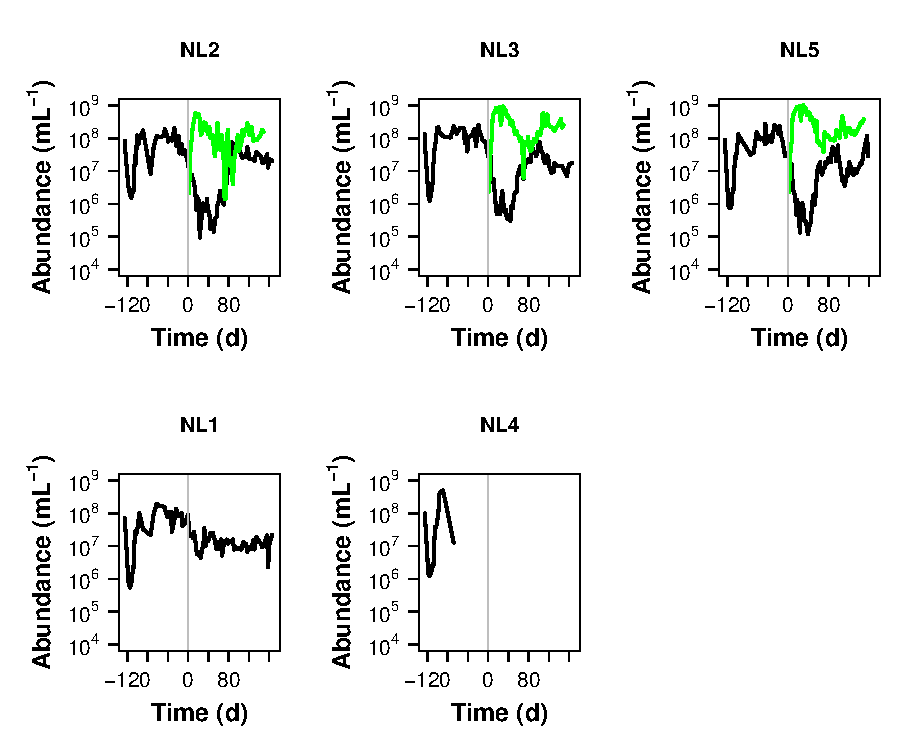
\includegraphics{analysis_ecoevostoich_files/figure-latex/unnamed-chunk-2-1.pdf}
\caption{Individul N-Limited chemostat replicates. Chemostats NL2, NL3,
and NL5 contained both \emph{Synechococcus} (black) and SRIM8 phage
(green) while chemostats NL1 and NL4 contained only
\emph{Synechococcus}. Chemostat NL4 was lost due to fungal contamination
prior to phage addition.}
\end{figure}

\newpage

\begin{figure}[htbp]
\centering
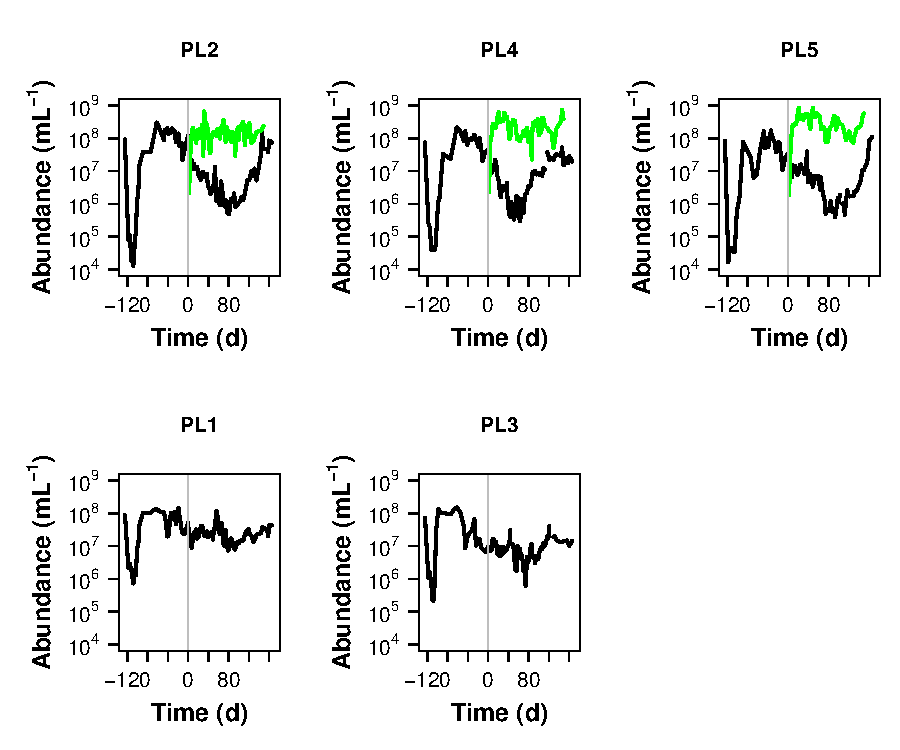
\includegraphics{analysis_ecoevostoich_files/figure-latex/unnamed-chunk-3-1.pdf}
\caption{Individul P-Limited chemostat replicates. Chemostats PL2, PL4,
and PL5 contained both \emph{Synechococcus} (black) and SRIM8 phage
(green) while chemostats PL1 and PL3 contained only
\emph{Synechococcus}.}
\end{figure}

\newpage

\subsubsection{Chemostat phase plane
diagrams}\label{chemostat-phase-plane-diagrams}

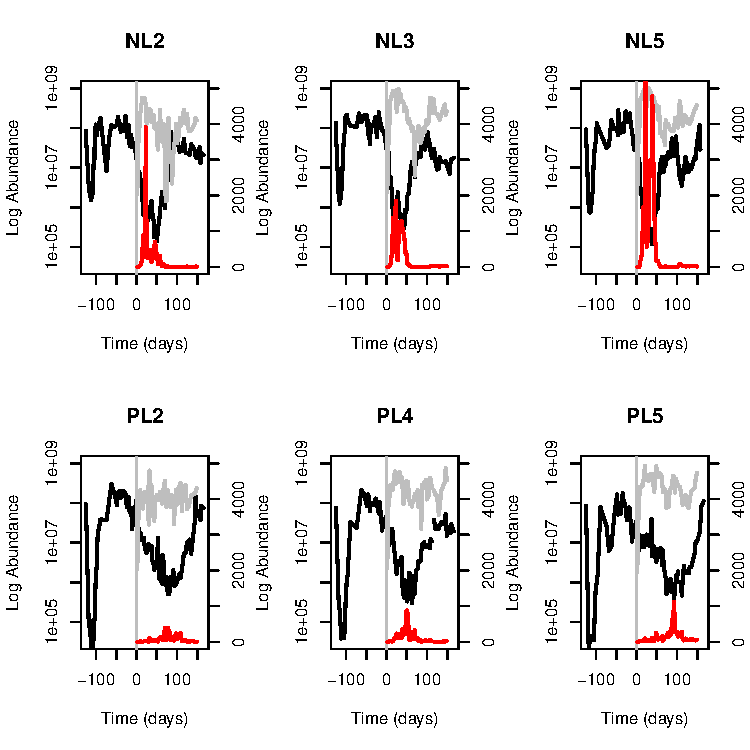
\includegraphics{analysis_ecoevostoich_files/figure-latex/unnamed-chunk-4-1.pdf}
\newpage

\subsection{Treatment-level
comparisons}\label{treatment-level-comparisons}

\begin{figure}[htbp]
\centering
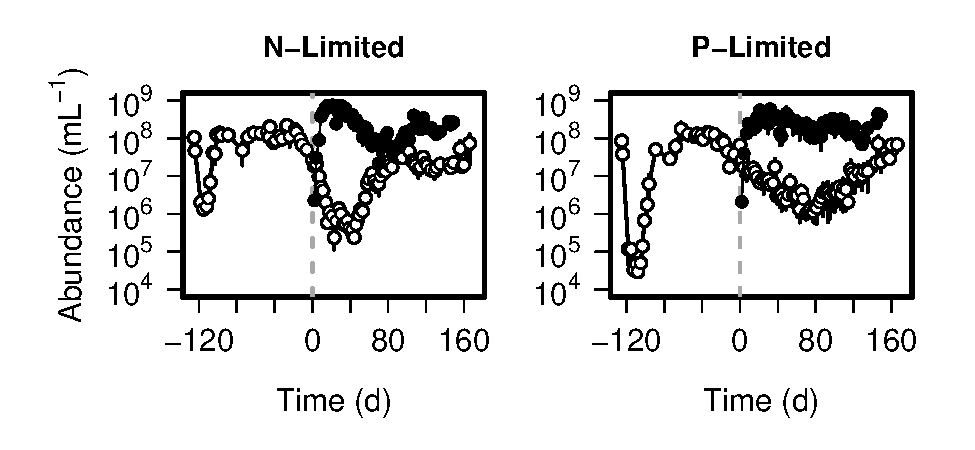
\includegraphics{analysis_ecoevostoich_files/figure-latex/unnamed-chunk-6-1.pdf}
\caption{Average population dynamics of Synechococcus (white) and SRIM8
phage (black) in N-limited and P-limited nutrient treatments. The dashed
line at day 0 indicates the time in which phage were added to the
chemostat system.}
\end{figure}

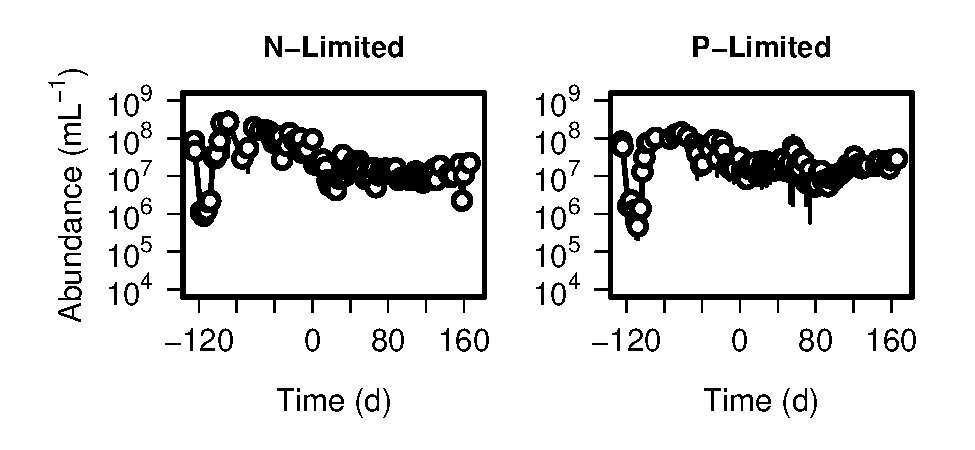
\includegraphics{analysis_ecoevostoich_files/figure-latex/unnamed-chunk-7-1.pdf}
\newpage

\subsubsection{Heteroskedaskicity
(skewness)}\label{heteroskedaskicity-skewness}

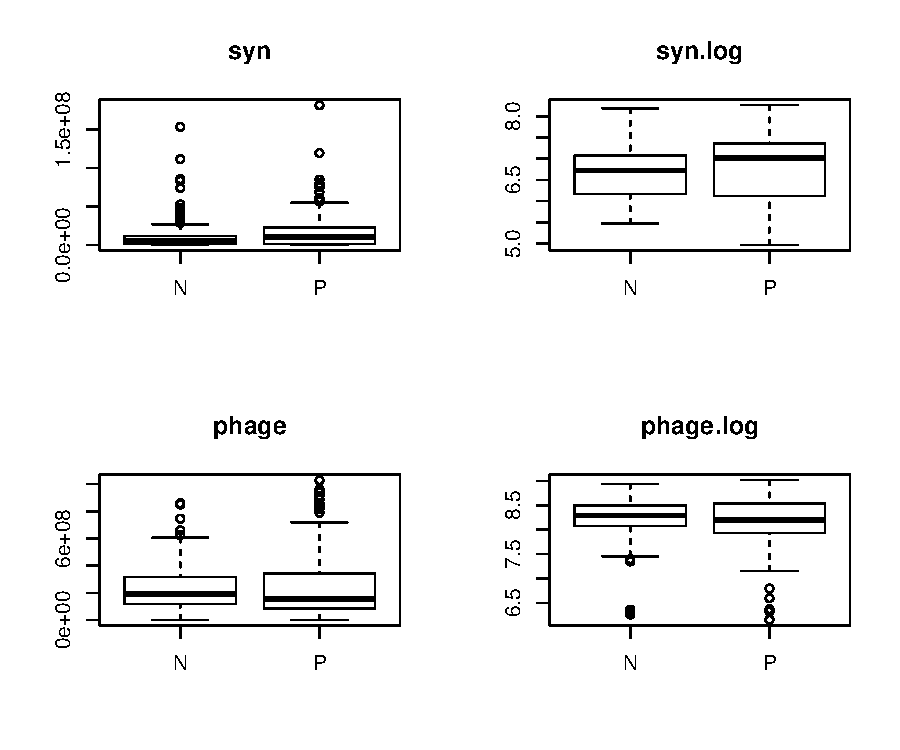
\includegraphics{analysis_ecoevostoich_files/figure-latex/unnamed-chunk-8-1.pdf}

\newpage

\subsubsection{Reapeated Measures ANOVA
(RMANOVA)}\label{reapeated-measures-anova-rmanova}

\textbf{+Ph \emph{Synechococcus} and phage}

\begin{longtable}[]{@{}ccccc@{}}
\caption{RMANOVA table for SRIM8 phage}\tabularnewline
\toprule
\begin{minipage}[b]{0.21\columnwidth}\centering\strut
~\strut
\end{minipage} & \begin{minipage}[b]{0.10\columnwidth}\centering\strut
numDF\strut
\end{minipage} & \begin{minipage}[b]{0.10\columnwidth}\centering\strut
denDF\strut
\end{minipage} & \begin{minipage}[b]{0.12\columnwidth}\centering\strut
F-value\strut
\end{minipage} & \begin{minipage}[b]{0.12\columnwidth}\centering\strut
p-value\strut
\end{minipage}\tabularnewline
\midrule
\endfirsthead
\toprule
\begin{minipage}[b]{0.21\columnwidth}\centering\strut
~\strut
\end{minipage} & \begin{minipage}[b]{0.10\columnwidth}\centering\strut
numDF\strut
\end{minipage} & \begin{minipage}[b]{0.10\columnwidth}\centering\strut
denDF\strut
\end{minipage} & \begin{minipage}[b]{0.12\columnwidth}\centering\strut
F-value\strut
\end{minipage} & \begin{minipage}[b]{0.12\columnwidth}\centering\strut
p-value\strut
\end{minipage}\tabularnewline
\midrule
\endhead
\begin{minipage}[t]{0.21\columnwidth}\centering\strut
\textbf{(Intercept)}\strut
\end{minipage} & \begin{minipage}[t]{0.10\columnwidth}\centering\strut
1\strut
\end{minipage} & \begin{minipage}[t]{0.10\columnwidth}\centering\strut
230\strut
\end{minipage} & \begin{minipage}[t]{0.12\columnwidth}\centering\strut
14010\strut
\end{minipage} & \begin{minipage}[t]{0.12\columnwidth}\centering\strut
0\strut
\end{minipage}\tabularnewline
\begin{minipage}[t]{0.21\columnwidth}\centering\strut
\textbf{lim}\strut
\end{minipage} & \begin{minipage}[t]{0.10\columnwidth}\centering\strut
1\strut
\end{minipage} & \begin{minipage}[t]{0.10\columnwidth}\centering\strut
4\strut
\end{minipage} & \begin{minipage}[t]{0.12\columnwidth}\centering\strut
0.3592\strut
\end{minipage} & \begin{minipage}[t]{0.12\columnwidth}\centering\strut
0.5812\strut
\end{minipage}\tabularnewline
\begin{minipage}[t]{0.21\columnwidth}\centering\strut
\textbf{day.fac}\strut
\end{minipage} & \begin{minipage}[t]{0.10\columnwidth}\centering\strut
58\strut
\end{minipage} & \begin{minipage}[t]{0.10\columnwidth}\centering\strut
230\strut
\end{minipage} & \begin{minipage}[t]{0.12\columnwidth}\centering\strut
10.22\strut
\end{minipage} & \begin{minipage}[t]{0.12\columnwidth}\centering\strut
0\strut
\end{minipage}\tabularnewline
\begin{minipage}[t]{0.21\columnwidth}\centering\strut
\textbf{lim:day.fac}\strut
\end{minipage} & \begin{minipage}[t]{0.10\columnwidth}\centering\strut
58\strut
\end{minipage} & \begin{minipage}[t]{0.10\columnwidth}\centering\strut
230\strut
\end{minipage} & \begin{minipage}[t]{0.12\columnwidth}\centering\strut
2.588\strut
\end{minipage} & \begin{minipage}[t]{0.12\columnwidth}\centering\strut
2.771e-07\strut
\end{minipage}\tabularnewline
\bottomrule
\end{longtable}

\begin{longtable}[]{@{}ccccc@{}}
\caption{RMANOVA table for +Ph Synechococcus}\tabularnewline
\toprule
\begin{minipage}[b]{0.21\columnwidth}\centering\strut
~\strut
\end{minipage} & \begin{minipage}[b]{0.10\columnwidth}\centering\strut
numDF\strut
\end{minipage} & \begin{minipage}[b]{0.10\columnwidth}\centering\strut
denDF\strut
\end{minipage} & \begin{minipage}[b]{0.12\columnwidth}\centering\strut
F-value\strut
\end{minipage} & \begin{minipage}[b]{0.12\columnwidth}\centering\strut
p-value\strut
\end{minipage}\tabularnewline
\midrule
\endfirsthead
\toprule
\begin{minipage}[b]{0.21\columnwidth}\centering\strut
~\strut
\end{minipage} & \begin{minipage}[b]{0.10\columnwidth}\centering\strut
numDF\strut
\end{minipage} & \begin{minipage}[b]{0.10\columnwidth}\centering\strut
denDF\strut
\end{minipage} & \begin{minipage}[b]{0.12\columnwidth}\centering\strut
F-value\strut
\end{minipage} & \begin{minipage}[b]{0.12\columnwidth}\centering\strut
p-value\strut
\end{minipage}\tabularnewline
\midrule
\endhead
\begin{minipage}[t]{0.21\columnwidth}\centering\strut
\textbf{(Intercept)}\strut
\end{minipage} & \begin{minipage}[t]{0.10\columnwidth}\centering\strut
1\strut
\end{minipage} & \begin{minipage}[t]{0.10\columnwidth}\centering\strut
245\strut
\end{minipage} & \begin{minipage}[t]{0.12\columnwidth}\centering\strut
12432\strut
\end{minipage} & \begin{minipage}[t]{0.12\columnwidth}\centering\strut
0\strut
\end{minipage}\tabularnewline
\begin{minipage}[t]{0.21\columnwidth}\centering\strut
\textbf{lim}\strut
\end{minipage} & \begin{minipage}[t]{0.10\columnwidth}\centering\strut
1\strut
\end{minipage} & \begin{minipage}[t]{0.10\columnwidth}\centering\strut
4\strut
\end{minipage} & \begin{minipage}[t]{0.12\columnwidth}\centering\strut
0.5225\strut
\end{minipage} & \begin{minipage}[t]{0.12\columnwidth}\centering\strut
0.5098\strut
\end{minipage}\tabularnewline
\begin{minipage}[t]{0.21\columnwidth}\centering\strut
\textbf{day.fac}\strut
\end{minipage} & \begin{minipage}[t]{0.10\columnwidth}\centering\strut
62\strut
\end{minipage} & \begin{minipage}[t]{0.10\columnwidth}\centering\strut
245\strut
\end{minipage} & \begin{minipage}[t]{0.12\columnwidth}\centering\strut
3.354\strut
\end{minipage} & \begin{minipage}[t]{0.12\columnwidth}\centering\strut
1.14e-11\strut
\end{minipage}\tabularnewline
\begin{minipage}[t]{0.21\columnwidth}\centering\strut
\textbf{lim:day.fac}\strut
\end{minipage} & \begin{minipage}[t]{0.10\columnwidth}\centering\strut
62\strut
\end{minipage} & \begin{minipage}[t]{0.10\columnwidth}\centering\strut
245\strut
\end{minipage} & \begin{minipage}[t]{0.12\columnwidth}\centering\strut
2.437\strut
\end{minipage} & \begin{minipage}[t]{0.12\columnwidth}\centering\strut
6.993e-07\strut
\end{minipage}\tabularnewline
\bottomrule
\end{longtable}

\begin{longtable}[]{@{}ccccc@{}}
\caption{RMANOVA table comparison between -Ph and +Ph
Synechococcus}\tabularnewline
\toprule
\begin{minipage}[b]{0.27\columnwidth}\centering\strut
~\strut
\end{minipage} & \begin{minipage}[b]{0.10\columnwidth}\centering\strut
numDF\strut
\end{minipage} & \begin{minipage}[b]{0.10\columnwidth}\centering\strut
denDF\strut
\end{minipage} & \begin{minipage}[b]{0.12\columnwidth}\centering\strut
F-value\strut
\end{minipage} & \begin{minipage}[b]{0.12\columnwidth}\centering\strut
p-value\strut
\end{minipage}\tabularnewline
\midrule
\endfirsthead
\toprule
\begin{minipage}[b]{0.27\columnwidth}\centering\strut
~\strut
\end{minipage} & \begin{minipage}[b]{0.10\columnwidth}\centering\strut
numDF\strut
\end{minipage} & \begin{minipage}[b]{0.10\columnwidth}\centering\strut
denDF\strut
\end{minipage} & \begin{minipage}[b]{0.12\columnwidth}\centering\strut
F-value\strut
\end{minipage} & \begin{minipage}[b]{0.12\columnwidth}\centering\strut
p-value\strut
\end{minipage}\tabularnewline
\midrule
\endhead
\begin{minipage}[t]{0.27\columnwidth}\centering\strut
\textbf{(Intercept)}\strut
\end{minipage} & \begin{minipage}[t]{0.10\columnwidth}\centering\strut
1\strut
\end{minipage} & \begin{minipage}[t]{0.10\columnwidth}\centering\strut
305\strut
\end{minipage} & \begin{minipage}[t]{0.12\columnwidth}\centering\strut
19415\strut
\end{minipage} & \begin{minipage}[t]{0.12\columnwidth}\centering\strut
0\strut
\end{minipage}\tabularnewline
\begin{minipage}[t]{0.27\columnwidth}\centering\strut
\textbf{lim}\strut
\end{minipage} & \begin{minipage}[t]{0.10\columnwidth}\centering\strut
1\strut
\end{minipage} & \begin{minipage}[t]{0.10\columnwidth}\centering\strut
5\strut
\end{minipage} & \begin{minipage}[t]{0.12\columnwidth}\centering\strut
0.002236\strut
\end{minipage} & \begin{minipage}[t]{0.12\columnwidth}\centering\strut
0.9641\strut
\end{minipage}\tabularnewline
\begin{minipage}[t]{0.27\columnwidth}\centering\strut
\textbf{day.fac}\strut
\end{minipage} & \begin{minipage}[t]{0.10\columnwidth}\centering\strut
62\strut
\end{minipage} & \begin{minipage}[t]{0.10\columnwidth}\centering\strut
305\strut
\end{minipage} & \begin{minipage}[t]{0.12\columnwidth}\centering\strut
2.87\strut
\end{minipage} & \begin{minipage}[t]{0.12\columnwidth}\centering\strut
1.107e-09\strut
\end{minipage}\tabularnewline
\begin{minipage}[t]{0.27\columnwidth}\centering\strut
\textbf{type}\strut
\end{minipage} & \begin{minipage}[t]{0.10\columnwidth}\centering\strut
1\strut
\end{minipage} & \begin{minipage}[t]{0.10\columnwidth}\centering\strut
5\strut
\end{minipage} & \begin{minipage}[t]{0.12\columnwidth}\centering\strut
8.787\strut
\end{minipage} & \begin{minipage}[t]{0.12\columnwidth}\centering\strut
0.03136\strut
\end{minipage}\tabularnewline
\begin{minipage}[t]{0.27\columnwidth}\centering\strut
\textbf{lim:day.fac}\strut
\end{minipage} & \begin{minipage}[t]{0.10\columnwidth}\centering\strut
62\strut
\end{minipage} & \begin{minipage}[t]{0.10\columnwidth}\centering\strut
305\strut
\end{minipage} & \begin{minipage}[t]{0.12\columnwidth}\centering\strut
2.354\strut
\end{minipage} & \begin{minipage}[t]{0.12\columnwidth}\centering\strut
8.796e-07\strut
\end{minipage}\tabularnewline
\begin{minipage}[t]{0.27\columnwidth}\centering\strut
\textbf{lim:type}\strut
\end{minipage} & \begin{minipage}[t]{0.10\columnwidth}\centering\strut
1\strut
\end{minipage} & \begin{minipage}[t]{0.10\columnwidth}\centering\strut
5\strut
\end{minipage} & \begin{minipage}[t]{0.12\columnwidth}\centering\strut
0.3204\strut
\end{minipage} & \begin{minipage}[t]{0.12\columnwidth}\centering\strut
0.5958\strut
\end{minipage}\tabularnewline
\begin{minipage}[t]{0.27\columnwidth}\centering\strut
\textbf{day.fac:type}\strut
\end{minipage} & \begin{minipage}[t]{0.10\columnwidth}\centering\strut
62\strut
\end{minipage} & \begin{minipage}[t]{0.10\columnwidth}\centering\strut
305\strut
\end{minipage} & \begin{minipage}[t]{0.12\columnwidth}\centering\strut
1.244\strut
\end{minipage} & \begin{minipage}[t]{0.12\columnwidth}\centering\strut
0.1198\strut
\end{minipage}\tabularnewline
\begin{minipage}[t]{0.27\columnwidth}\centering\strut
\textbf{lim:day.fac:type}\strut
\end{minipage} & \begin{minipage}[t]{0.10\columnwidth}\centering\strut
62\strut
\end{minipage} & \begin{minipage}[t]{0.10\columnwidth}\centering\strut
305\strut
\end{minipage} & \begin{minipage}[t]{0.12\columnwidth}\centering\strut
1.121\strut
\end{minipage} & \begin{minipage}[t]{0.12\columnwidth}\centering\strut
0.2639\strut
\end{minipage}\tabularnewline
\bottomrule
\end{longtable}

\begin{longtable}[]{@{}ccccc@{}}
\caption{RMANOVA for -Ph Synechococcus}\tabularnewline
\toprule
\begin{minipage}[b]{0.21\columnwidth}\centering\strut
~\strut
\end{minipage} & \begin{minipage}[b]{0.10\columnwidth}\centering\strut
numDF\strut
\end{minipage} & \begin{minipage}[b]{0.10\columnwidth}\centering\strut
denDF\strut
\end{minipage} & \begin{minipage}[b]{0.12\columnwidth}\centering\strut
F-value\strut
\end{minipage} & \begin{minipage}[b]{0.12\columnwidth}\centering\strut
p-value\strut
\end{minipage}\tabularnewline
\midrule
\endfirsthead
\toprule
\begin{minipage}[b]{0.21\columnwidth}\centering\strut
~\strut
\end{minipage} & \begin{minipage}[b]{0.10\columnwidth}\centering\strut
numDF\strut
\end{minipage} & \begin{minipage}[b]{0.10\columnwidth}\centering\strut
denDF\strut
\end{minipage} & \begin{minipage}[b]{0.12\columnwidth}\centering\strut
F-value\strut
\end{minipage} & \begin{minipage}[b]{0.12\columnwidth}\centering\strut
p-value\strut
\end{minipage}\tabularnewline
\midrule
\endhead
\begin{minipage}[t]{0.21\columnwidth}\centering\strut
\textbf{(Intercept)}\strut
\end{minipage} & \begin{minipage}[t]{0.10\columnwidth}\centering\strut
1\strut
\end{minipage} & \begin{minipage}[t]{0.10\columnwidth}\centering\strut
60\strut
\end{minipage} & \begin{minipage}[t]{0.12\columnwidth}\centering\strut
1629\strut
\end{minipage} & \begin{minipage}[t]{0.12\columnwidth}\centering\strut
0\strut
\end{minipage}\tabularnewline
\begin{minipage}[t]{0.21\columnwidth}\centering\strut
\textbf{lim}\strut
\end{minipage} & \begin{minipage}[t]{0.10\columnwidth}\centering\strut
1\strut
\end{minipage} & \begin{minipage}[t]{0.10\columnwidth}\centering\strut
1\strut
\end{minipage} & \begin{minipage}[t]{0.12\columnwidth}\centering\strut
0.01077\strut
\end{minipage} & \begin{minipage}[t]{0.12\columnwidth}\centering\strut
0.9342\strut
\end{minipage}\tabularnewline
\begin{minipage}[t]{0.21\columnwidth}\centering\strut
\textbf{day.fac}\strut
\end{minipage} & \begin{minipage}[t]{0.10\columnwidth}\centering\strut
62\strut
\end{minipage} & \begin{minipage}[t]{0.10\columnwidth}\centering\strut
60\strut
\end{minipage} & \begin{minipage}[t]{0.12\columnwidth}\centering\strut
0.9176\strut
\end{minipage} & \begin{minipage}[t]{0.12\columnwidth}\centering\strut
0.6315\strut
\end{minipage}\tabularnewline
\begin{minipage}[t]{0.21\columnwidth}\centering\strut
\textbf{lim:day.fac}\strut
\end{minipage} & \begin{minipage}[t]{0.10\columnwidth}\centering\strut
62\strut
\end{minipage} & \begin{minipage}[t]{0.10\columnwidth}\centering\strut
60\strut
\end{minipage} & \begin{minipage}[t]{0.12\columnwidth}\centering\strut
0.9089\strut
\end{minipage} & \begin{minipage}[t]{0.12\columnwidth}\centering\strut
0.6454\strut
\end{minipage}\tabularnewline
\bottomrule
\end{longtable}

\newpage

\subsubsection{Temporal autocorrelation}\label{temporal-autocorrelation}

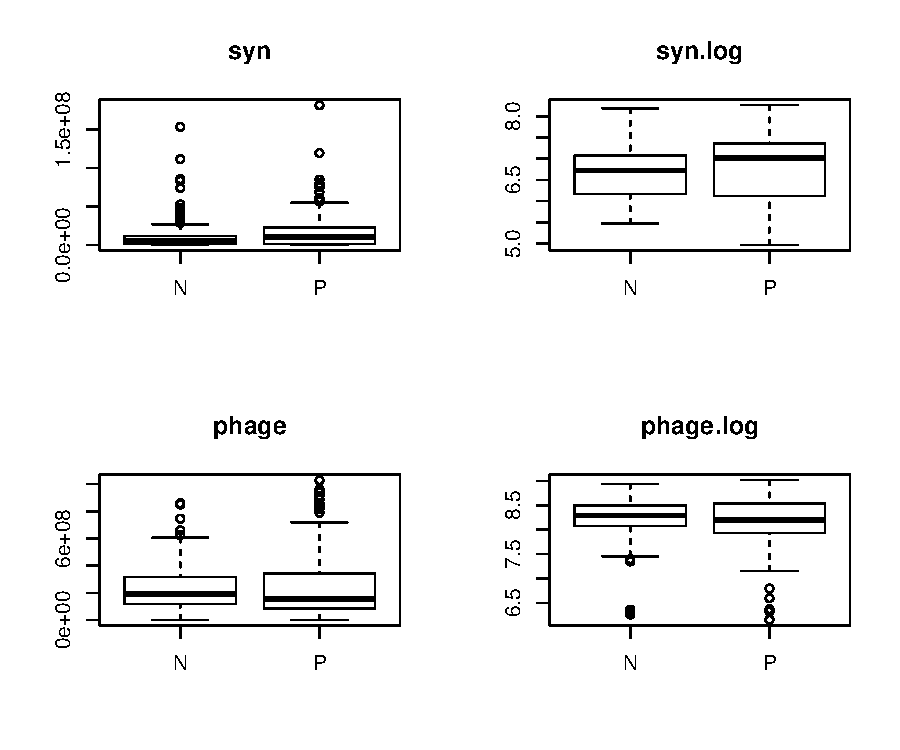
\includegraphics{analysis_ecoevostoich_files/figure-latex/unnamed-chunk-12-1.pdf}
\emph{NOTE}: Cross-correlation analyses and RMANOVA were also completed
in SAS

\newpage

\subsection{Despcriptive statistics}\label{despcriptive-statistics}

\begin{longtable}[]{@{}cccccc@{}}
\toprule
\begin{minipage}[b]{0.07\columnwidth}\centering\strut
lim\strut
\end{minipage} & \begin{minipage}[b]{0.07\columnwidth}\centering\strut
cID\strut
\end{minipage} & \begin{minipage}[b]{0.12\columnwidth}\centering\strut
microbe\strut
\end{minipage} & \begin{minipage}[b]{0.10\columnwidth}\centering\strut
mean\strut
\end{minipage} & \begin{minipage}[b]{0.12\columnwidth}\centering\strut
var\strut
\end{minipage} & \begin{minipage}[b]{0.12\columnwidth}\centering\strut
sem\strut
\end{minipage}\tabularnewline
\midrule
\endhead
\begin{minipage}[t]{0.07\columnwidth}\centering\strut
N\strut
\end{minipage} & \begin{minipage}[t]{0.07\columnwidth}\centering\strut
NL1\strut
\end{minipage} & \begin{minipage}[t]{0.12\columnwidth}\centering\strut
Syn\strut
\end{minipage} & \begin{minipage}[t]{0.10\columnwidth}\centering\strut
13134483\strut
\end{minipage} & \begin{minipage}[t]{0.12\columnwidth}\centering\strut
4.093e+13\strut
\end{minipage} & \begin{minipage}[t]{0.12\columnwidth}\centering\strut
3693536\strut
\end{minipage}\tabularnewline
\begin{minipage}[t]{0.07\columnwidth}\centering\strut
P\strut
\end{minipage} & \begin{minipage}[t]{0.07\columnwidth}\centering\strut
PL1\strut
\end{minipage} & \begin{minipage}[t]{0.12\columnwidth}\centering\strut
Syn\strut
\end{minipage} & \begin{minipage}[t]{0.10\columnwidth}\centering\strut
25428955\strut
\end{minipage} & \begin{minipage}[t]{0.12\columnwidth}\centering\strut
3.159e+14\strut
\end{minipage} & \begin{minipage}[t]{0.12\columnwidth}\centering\strut
10261999\strut
\end{minipage}\tabularnewline
\begin{minipage}[t]{0.07\columnwidth}\centering\strut
P\strut
\end{minipage} & \begin{minipage}[t]{0.07\columnwidth}\centering\strut
PL3\strut
\end{minipage} & \begin{minipage}[t]{0.12\columnwidth}\centering\strut
Syn\strut
\end{minipage} & \begin{minipage}[t]{0.10\columnwidth}\centering\strut
9864044\strut
\end{minipage} & \begin{minipage}[t]{0.12\columnwidth}\centering\strut
4.838e+13\strut
\end{minipage} & \begin{minipage}[t]{0.12\columnwidth}\centering\strut
4015664\strut
\end{minipage}\tabularnewline
\begin{minipage}[t]{0.07\columnwidth}\centering\strut
NA\strut
\end{minipage} & \begin{minipage}[t]{0.07\columnwidth}\centering\strut
NA\strut
\end{minipage} & \begin{minipage}[t]{0.12\columnwidth}\centering\strut
NA\strut
\end{minipage} & \begin{minipage}[t]{0.10\columnwidth}\centering\strut
NA\strut
\end{minipage} & \begin{minipage}[t]{0.12\columnwidth}\centering\strut
NA\strut
\end{minipage} & \begin{minipage}[t]{0.12\columnwidth}\centering\strut
NA\strut
\end{minipage}\tabularnewline
\begin{minipage}[t]{0.07\columnwidth}\centering\strut
NA\strut
\end{minipage} & \begin{minipage}[t]{0.07\columnwidth}\centering\strut
NA\strut
\end{minipage} & \begin{minipage}[t]{0.12\columnwidth}\centering\strut
NA\strut
\end{minipage} & \begin{minipage}[t]{0.10\columnwidth}\centering\strut
NA\strut
\end{minipage} & \begin{minipage}[t]{0.12\columnwidth}\centering\strut
NA\strut
\end{minipage} & \begin{minipage}[t]{0.12\columnwidth}\centering\strut
NA\strut
\end{minipage}\tabularnewline
\begin{minipage}[t]{0.07\columnwidth}\centering\strut
NA\strut
\end{minipage} & \begin{minipage}[t]{0.07\columnwidth}\centering\strut
NA\strut
\end{minipage} & \begin{minipage}[t]{0.12\columnwidth}\centering\strut
NA\strut
\end{minipage} & \begin{minipage}[t]{0.10\columnwidth}\centering\strut
NA\strut
\end{minipage} & \begin{minipage}[t]{0.12\columnwidth}\centering\strut
NA\strut
\end{minipage} & \begin{minipage}[t]{0.12\columnwidth}\centering\strut
NA\strut
\end{minipage}\tabularnewline
\begin{minipage}[t]{0.07\columnwidth}\centering\strut
NA\strut
\end{minipage} & \begin{minipage}[t]{0.07\columnwidth}\centering\strut
NA\strut
\end{minipage} & \begin{minipage}[t]{0.12\columnwidth}\centering\strut
NA\strut
\end{minipage} & \begin{minipage}[t]{0.10\columnwidth}\centering\strut
NA\strut
\end{minipage} & \begin{minipage}[t]{0.12\columnwidth}\centering\strut
NA\strut
\end{minipage} & \begin{minipage}[t]{0.12\columnwidth}\centering\strut
NA\strut
\end{minipage}\tabularnewline
\begin{minipage}[t]{0.07\columnwidth}\centering\strut
NA\strut
\end{minipage} & \begin{minipage}[t]{0.07\columnwidth}\centering\strut
NA\strut
\end{minipage} & \begin{minipage}[t]{0.12\columnwidth}\centering\strut
NA\strut
\end{minipage} & \begin{minipage}[t]{0.10\columnwidth}\centering\strut
NA\strut
\end{minipage} & \begin{minipage}[t]{0.12\columnwidth}\centering\strut
NA\strut
\end{minipage} & \begin{minipage}[t]{0.12\columnwidth}\centering\strut
NA\strut
\end{minipage}\tabularnewline
\begin{minipage}[t]{0.07\columnwidth}\centering\strut
NA\strut
\end{minipage} & \begin{minipage}[t]{0.07\columnwidth}\centering\strut
NA\strut
\end{minipage} & \begin{minipage}[t]{0.12\columnwidth}\centering\strut
NA\strut
\end{minipage} & \begin{minipage}[t]{0.10\columnwidth}\centering\strut
NA\strut
\end{minipage} & \begin{minipage}[t]{0.12\columnwidth}\centering\strut
NA\strut
\end{minipage} & \begin{minipage}[t]{0.12\columnwidth}\centering\strut
NA\strut
\end{minipage}\tabularnewline
\begin{minipage}[t]{0.07\columnwidth}\centering\strut
NA\strut
\end{minipage} & \begin{minipage}[t]{0.07\columnwidth}\centering\strut
NA\strut
\end{minipage} & \begin{minipage}[t]{0.12\columnwidth}\centering\strut
NA\strut
\end{minipage} & \begin{minipage}[t]{0.10\columnwidth}\centering\strut
NA\strut
\end{minipage} & \begin{minipage}[t]{0.12\columnwidth}\centering\strut
NA\strut
\end{minipage} & \begin{minipage}[t]{0.12\columnwidth}\centering\strut
NA\strut
\end{minipage}\tabularnewline
\begin{minipage}[t]{0.07\columnwidth}\centering\strut
NA\strut
\end{minipage} & \begin{minipage}[t]{0.07\columnwidth}\centering\strut
NA\strut
\end{minipage} & \begin{minipage}[t]{0.12\columnwidth}\centering\strut
NA\strut
\end{minipage} & \begin{minipage}[t]{0.10\columnwidth}\centering\strut
NA\strut
\end{minipage} & \begin{minipage}[t]{0.12\columnwidth}\centering\strut
NA\strut
\end{minipage} & \begin{minipage}[t]{0.12\columnwidth}\centering\strut
NA\strut
\end{minipage}\tabularnewline
\begin{minipage}[t]{0.07\columnwidth}\centering\strut
NA\strut
\end{minipage} & \begin{minipage}[t]{0.07\columnwidth}\centering\strut
NA\strut
\end{minipage} & \begin{minipage}[t]{0.12\columnwidth}\centering\strut
NA\strut
\end{minipage} & \begin{minipage}[t]{0.10\columnwidth}\centering\strut
NA\strut
\end{minipage} & \begin{minipage}[t]{0.12\columnwidth}\centering\strut
NA\strut
\end{minipage} & \begin{minipage}[t]{0.12\columnwidth}\centering\strut
NA\strut
\end{minipage}\tabularnewline
\bottomrule
\end{longtable}

\begin{longtable}[]{@{}cccccc@{}}
\toprule
\begin{minipage}[b]{0.12\columnwidth}\centering\strut
Limitation\strut
\end{minipage} & \begin{minipage}[b]{0.11\columnwidth}\centering\strut
Treatment\strut
\end{minipage} & \begin{minipage}[b]{0.15\columnwidth}\centering\strut
Synechococcus mean densitiy (+/- SEM)\strut
\end{minipage} & \begin{minipage}[b]{0.16\columnwidth}\centering\strut
Synechococcus mean stability\strut
\end{minipage} & \begin{minipage}[b]{0.16\columnwidth}\centering\strut
Phage mean density (+/- SEM)\strut
\end{minipage} & \begin{minipage}[b]{0.11\columnwidth}\centering\strut
Phage mean stability\strut
\end{minipage}\tabularnewline
\midrule
\endhead
\begin{minipage}[t]{0.12\columnwidth}\centering\strut
N\strut
\end{minipage} & \begin{minipage}[t]{0.11\columnwidth}\centering\strut
Control\strut
\end{minipage} & \begin{minipage}[t]{0.15\columnwidth}\centering\strut
1.3e+07(4e+06)\strut
\end{minipage} & \begin{minipage}[t]{0.16\columnwidth}\centering\strut
2.1\strut
\end{minipage} & \begin{minipage}[t]{0.16\columnwidth}\centering\strut
NaN(NA)\strut
\end{minipage} & \begin{minipage}[t]{0.11\columnwidth}\centering\strut
NA\strut
\end{minipage}\tabularnewline
\begin{minipage}[t]{0.12\columnwidth}\centering\strut
N\strut
\end{minipage} & \begin{minipage}[t]{0.11\columnwidth}\centering\strut
Infect\strut
\end{minipage} & \begin{minipage}[t]{0.15\columnwidth}\centering\strut
1.7e+07(1e+07)\strut
\end{minipage} & \begin{minipage}[t]{0.16\columnwidth}\centering\strut
0.75\strut
\end{minipage} & \begin{minipage}[t]{0.16\columnwidth}\centering\strut
2.5e+08(1.4e+08)\strut
\end{minipage} & \begin{minipage}[t]{0.11\columnwidth}\centering\strut
1\strut
\end{minipage}\tabularnewline
\begin{minipage}[t]{0.12\columnwidth}\centering\strut
P\strut
\end{minipage} & \begin{minipage}[t]{0.11\columnwidth}\centering\strut
Control\strut
\end{minipage} & \begin{minipage}[t]{0.15\columnwidth}\centering\strut
1.8e+07(9e+06)\strut
\end{minipage} & \begin{minipage}[t]{0.16\columnwidth}\centering\strut
1.1\strut
\end{minipage} & \begin{minipage}[t]{0.16\columnwidth}\centering\strut
NaN(NA)\strut
\end{minipage} & \begin{minipage}[t]{0.11\columnwidth}\centering\strut
NA\strut
\end{minipage}\tabularnewline
\begin{minipage}[t]{0.12\columnwidth}\centering\strut
P\strut
\end{minipage} & \begin{minipage}[t]{0.11\columnwidth}\centering\strut
Infect\strut
\end{minipage} & \begin{minipage}[t]{0.15\columnwidth}\centering\strut
1.1e+07(1e+07)\strut
\end{minipage} & \begin{minipage}[t]{0.16\columnwidth}\centering\strut
0.59\strut
\end{minipage} & \begin{minipage}[t]{0.16\columnwidth}\centering\strut
2.4e+08(9.5e+07)\strut
\end{minipage} & \begin{minipage}[t]{0.11\columnwidth}\centering\strut
1.5\strut
\end{minipage}\tabularnewline
\bottomrule
\end{longtable}

\begin{longtable}[]{@{}cccccc@{}}
\toprule
\begin{minipage}[b]{0.12\columnwidth}\centering\strut
Chemostat\strut
\end{minipage} & \begin{minipage}[b]{0.12\columnwidth}\centering\strut
Treatment\strut
\end{minipage} & \begin{minipage}[b]{0.16\columnwidth}\centering\strut
Synechococcus mean densitiy (+/- SEM)\strut
\end{minipage} & \begin{minipage}[b]{0.16\columnwidth}\centering\strut
Synechococcus mean stability\strut
\end{minipage} & \begin{minipage}[b]{0.17\columnwidth}\centering\strut
Phage mean density (+/- SEM)\strut
\end{minipage} & \begin{minipage}[b]{0.12\columnwidth}\centering\strut
Phage mean stability\strut
\end{minipage}\tabularnewline
\midrule
\endhead
\begin{minipage}[t]{0.12\columnwidth}\centering\strut
NL1\strut
\end{minipage} & \begin{minipage}[t]{0.12\columnwidth}\centering\strut
Control\strut
\end{minipage} & \begin{minipage}[t]{0.16\columnwidth}\centering\strut
1.3e+07(4e+06)\strut
\end{minipage} & \begin{minipage}[t]{0.16\columnwidth}\centering\strut
2.1\strut
\end{minipage} & \begin{minipage}[t]{0.17\columnwidth}\centering\strut
NaN(NA)\strut
\end{minipage} & \begin{minipage}[t]{0.12\columnwidth}\centering\strut
NA\strut
\end{minipage}\tabularnewline
\begin{minipage}[t]{0.12\columnwidth}\centering\strut
NL2\strut
\end{minipage} & \begin{minipage}[t]{0.12\columnwidth}\centering\strut
Infect\strut
\end{minipage} & \begin{minipage}[t]{0.16\columnwidth}\centering\strut
1.8e+07(1e+07)\strut
\end{minipage} & \begin{minipage}[t]{0.16\columnwidth}\centering\strut
0.84\strut
\end{minipage} & \begin{minipage}[t]{0.17\columnwidth}\centering\strut
1.5e+08(7.9e+07)\strut
\end{minipage} & \begin{minipage}[t]{0.12\columnwidth}\centering\strut
1.1\strut
\end{minipage}\tabularnewline
\begin{minipage}[t]{0.12\columnwidth}\centering\strut
NL3\strut
\end{minipage} & \begin{minipage}[t]{0.12\columnwidth}\centering\strut
Infect\strut
\end{minipage} & \begin{minipage}[t]{0.16\columnwidth}\centering\strut
1.6e+07(1e+07)\strut
\end{minipage} & \begin{minipage}[t]{0.16\columnwidth}\centering\strut
0.93\strut
\end{minipage} & \begin{minipage}[t]{0.17\columnwidth}\centering\strut
2.9e+08(1.5e+08)\strut
\end{minipage} & \begin{minipage}[t]{0.12\columnwidth}\centering\strut
1.2\strut
\end{minipage}\tabularnewline
\begin{minipage}[t]{0.12\columnwidth}\centering\strut
NL5\strut
\end{minipage} & \begin{minipage}[t]{0.12\columnwidth}\centering\strut
Infect\strut
\end{minipage} & \begin{minipage}[t]{0.16\columnwidth}\centering\strut
1.7e+07(2e+07)\strut
\end{minipage} & \begin{minipage}[t]{0.16\columnwidth}\centering\strut
0.59\strut
\end{minipage} & \begin{minipage}[t]{0.17\columnwidth}\centering\strut
3.1e+08(1.6e+08)\strut
\end{minipage} & \begin{minipage}[t]{0.12\columnwidth}\centering\strut
1.1\strut
\end{minipage}\tabularnewline
\begin{minipage}[t]{0.12\columnwidth}\centering\strut
PL1\strut
\end{minipage} & \begin{minipage}[t]{0.12\columnwidth}\centering\strut
Control\strut
\end{minipage} & \begin{minipage}[t]{0.16\columnwidth}\centering\strut
2.5e+07(1e+07)\strut
\end{minipage} & \begin{minipage}[t]{0.16\columnwidth}\centering\strut
1.4\strut
\end{minipage} & \begin{minipage}[t]{0.17\columnwidth}\centering\strut
NaN(NA)\strut
\end{minipage} & \begin{minipage}[t]{0.12\columnwidth}\centering\strut
NA\strut
\end{minipage}\tabularnewline
\begin{minipage}[t]{0.12\columnwidth}\centering\strut
PL2\strut
\end{minipage} & \begin{minipage}[t]{0.12\columnwidth}\centering\strut
Infect\strut
\end{minipage} & \begin{minipage}[t]{0.16\columnwidth}\centering\strut
1.3e+07(1e+07)\strut
\end{minipage} & \begin{minipage}[t]{0.16\columnwidth}\centering\strut
0.52\strut
\end{minipage} & \begin{minipage}[t]{0.17\columnwidth}\centering\strut
1.6e+08(5.9e+07)\strut
\end{minipage} & \begin{minipage}[t]{0.12\columnwidth}\centering\strut
1.6\strut
\end{minipage}\tabularnewline
\begin{minipage}[t]{0.12\columnwidth}\centering\strut
PL3\strut
\end{minipage} & \begin{minipage}[t]{0.12\columnwidth}\centering\strut
Control\strut
\end{minipage} & \begin{minipage}[t]{0.16\columnwidth}\centering\strut
9864044(4e+06)\strut
\end{minipage} & \begin{minipage}[t]{0.16\columnwidth}\centering\strut
1.4\strut
\end{minipage} & \begin{minipage}[t]{0.17\columnwidth}\centering\strut
NaN(NA)\strut
\end{minipage} & \begin{minipage}[t]{0.12\columnwidth}\centering\strut
NA\strut
\end{minipage}\tabularnewline
\begin{minipage}[t]{0.12\columnwidth}\centering\strut
PL4\strut
\end{minipage} & \begin{minipage}[t]{0.12\columnwidth}\centering\strut
Infect\strut
\end{minipage} & \begin{minipage}[t]{0.16\columnwidth}\centering\strut
1.1e+07(7e+06)\strut
\end{minipage} & \begin{minipage}[t]{0.16\columnwidth}\centering\strut
0.94\strut
\end{minipage} & \begin{minipage}[t]{0.17\columnwidth}\centering\strut
2.4e+08(8.8e+07)\strut
\end{minipage} & \begin{minipage}[t]{0.12\columnwidth}\centering\strut
1.6\strut
\end{minipage}\tabularnewline
\begin{minipage}[t]{0.12\columnwidth}\centering\strut
PL5\strut
\end{minipage} & \begin{minipage}[t]{0.12\columnwidth}\centering\strut
Infect\strut
\end{minipage} & \begin{minipage}[t]{0.16\columnwidth}\centering\strut
9399556(1e+07)\strut
\end{minipage} & \begin{minipage}[t]{0.16\columnwidth}\centering\strut
0.52\strut
\end{minipage} & \begin{minipage}[t]{0.17\columnwidth}\centering\strut
3.1e+08(1.1e+08)\strut
\end{minipage} & \begin{minipage}[t]{0.12\columnwidth}\centering\strut
1.6\strut
\end{minipage}\tabularnewline
\bottomrule
\end{longtable}

\newpage

\subsection{Topographic statistics}\label{topographic-statistics}

\begin{longtable}[]{@{}llllllll@{}}
\caption{Descriptive statistical summary of population data. (continued
below)}\tabularnewline
\toprule
\begin{minipage}[t]{0.08\columnwidth}\raggedright\strut
\textbf{lim}\strut
\end{minipage} & \begin{minipage}[t]{0.08\columnwidth}\raggedright\strut
\textbf{cID}\strut
\end{minipage} & \begin{minipage}[t]{0.13\columnwidth}\raggedright\strut
\textbf{microbe}\strut
\end{minipage} & \begin{minipage}[t]{0.09\columnwidth}\raggedright\strut
\textbf{mean}\strut
\end{minipage} & \begin{minipage}[t]{0.08\columnwidth}\raggedright\strut
\textbf{var}\strut
\end{minipage} & \begin{minipage}[t]{0.08\columnwidth}\raggedright\strut
\textbf{sem}\strut
\end{minipage} & \begin{minipage}[t]{0.09\columnwidth}\raggedright\strut
\textbf{stab}\strut
\end{minipage} & \begin{minipage}[t]{0.14\columnwidth}\raggedright\strut
\textbf{start.abd}\strut
\end{minipage}\tabularnewline
\bottomrule
\end{longtable}

\begin{longtable}[]{@{}lllll@{}}
\toprule
\begin{minipage}[t]{0.17\columnwidth}\raggedright\strut
\textbf{final.abd}\strut
\end{minipage} & \begin{minipage}[t]{0.14\columnwidth}\raggedright\strut
\textbf{min.day}\strut
\end{minipage} & \begin{minipage}[t]{0.14\columnwidth}\raggedright\strut
\textbf{min.abd}\strut
\end{minipage} & \begin{minipage}[t]{0.14\columnwidth}\raggedright\strut
\textbf{max.day}\strut
\end{minipage} & \begin{minipage}[t]{0.14\columnwidth}\raggedright\strut
\textbf{max.abd}\strut
\end{minipage}\tabularnewline
\bottomrule
\end{longtable}

\newpage

\section{Infection Dynamics: Does stoichiometry alter phenotypic
(co)evolution in cyanobacteria and
phage?}\label{infection-dynamics-does-stoichiometry-alter-phenotypic-coevolution-in-cyanobacteria-and-phage}

\textbf{Overview}: To examine how nutrient stoichiometry impact
evolutionary interactions, I collected cross-infectivity data from 96
phage and \textasciitilde{}200 \emph{Synechococcus} strains. Each
challenge was recorded based on cellular growth where lysis = 1
(i.e.~infectious interaction occured) or no lysis (i.e.~no evidence of
infection; cell line is resistant). This data was incorporated into
network-based metrics.

\subsection{Summary of Major Results}\label{summary-of-major-results-2}

\begin{enumerate}
\def\labelenumi{\arabic{enumi}.}
\tightlist
\item
  \textbf{Are temporal infection dynamics affected by stoichiometry?}
\item
  \textbf{Do community infection networks change as a result of the
  environment?}
\item
  \textbf{How are the dynamics affected? Through changes in overall
  resistance/infectivity? Changes in compositional resistance?}
\end{enumerate}

\newpage

\subsection{Degree of interaction}\label{degree-of-interaction}

\subsection{\texorpdfstring{\protect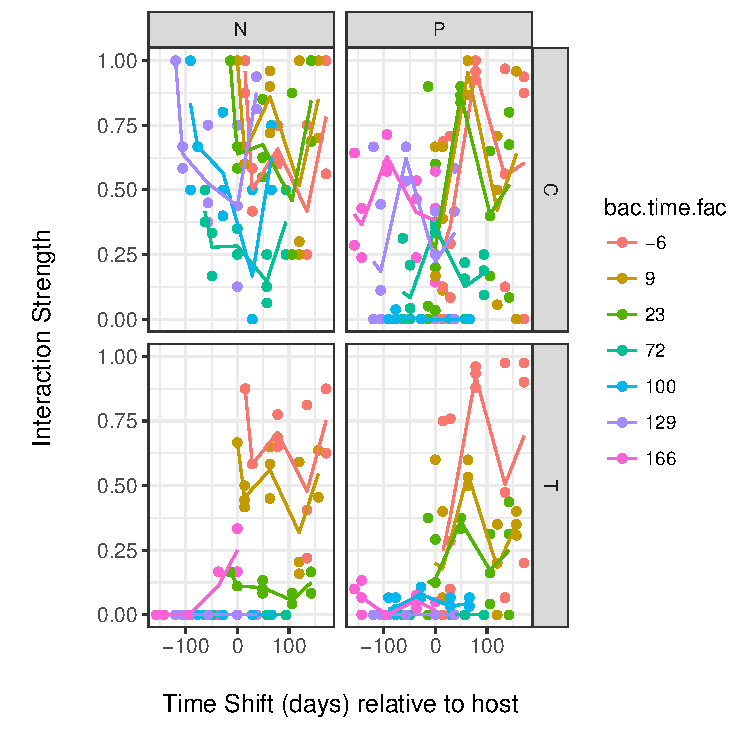
\includegraphics{analysis_ecoevostoich_files/figure-latex/unnamed-chunk-18-1.pdf}}{}}\label{section}

\begin{longtable}[]{@{}cccccc@{}}
\toprule
~ & Value & Std.Error & DF & t-value & p-value\tabularnewline
\midrule
\endhead
\textbf{(Intercept)} & 0.6284 & 0.03853 & 890 & 16.31 &
1.635e-52\tabularnewline
\bottomrule
\end{longtable}

\begin{verbatim}
     **trtT**           -0.4375     0.04353    5    -10.05   0.0001667

     **limP**           -0.2763     0.04541    5    -6.084   0.001735 

  **time.shift**       -0.0008488  0.0003838  890   -2.211    0.02726 

  **trtT:limP**          0.2379     0.05345    5     4.45    0.006701 
\end{verbatim}

\textbf{trtT:time.shift} 0.002118 0.0004238 890 4.997 7.002e-07

\textbf{limP:time.shift} 0.001718 0.0004391 890 3.912 9.853e-05

\subsection{\texorpdfstring{\textbf{trtT:limP:time.shift} -0.001685
0.0005044 890 -3.341
0.0008681}{trtT:limP:time.shift -0.001685 0.0005044 890 -3.341 0.0008681}}\label{trttlimptime.shift--0.001685-0.0005044-890--3.341-0.0008681}

\begin{longtable}[]{@{}ccccc@{}}
\caption{Fixed effects: inf.prob \textasciitilde{} trt * lim *
time.shift}\tabularnewline
\toprule
\begin{minipage}[b]{0.08\columnwidth}\centering\strut
Min\strut
\end{minipage} & \begin{minipage}[b]{0.10\columnwidth}\centering\strut
Q1\strut
\end{minipage} & \begin{minipage}[b]{0.10\columnwidth}\centering\strut
Med\strut
\end{minipage} & \begin{minipage}[b]{0.07\columnwidth}\centering\strut
Q3\strut
\end{minipage} & \begin{minipage}[b]{0.07\columnwidth}\centering\strut
Max\strut
\end{minipage}\tabularnewline
\midrule
\endfirsthead
\toprule
\begin{minipage}[b]{0.08\columnwidth}\centering\strut
Min\strut
\end{minipage} & \begin{minipage}[b]{0.10\columnwidth}\centering\strut
Q1\strut
\end{minipage} & \begin{minipage}[b]{0.10\columnwidth}\centering\strut
Med\strut
\end{minipage} & \begin{minipage}[b]{0.07\columnwidth}\centering\strut
Q3\strut
\end{minipage} & \begin{minipage}[b]{0.07\columnwidth}\centering\strut
Max\strut
\end{minipage}\tabularnewline
\midrule
\endhead
\begin{minipage}[t]{0.08\columnwidth}\centering\strut
-2.277\strut
\end{minipage} & \begin{minipage}[t]{0.10\columnwidth}\centering\strut
-0.7172\strut
\end{minipage} & \begin{minipage}[t]{0.10\columnwidth}\centering\strut
-0.2124\strut
\end{minipage} & \begin{minipage}[t]{0.07\columnwidth}\centering\strut
0.573\strut
\end{minipage} & \begin{minipage}[t]{0.07\columnwidth}\centering\strut
2.662\strut
\end{minipage}\tabularnewline
\bottomrule
\end{longtable}

\begin{longtable}[]{@{}cccc@{}}
\caption{Standardized Within-Group Residuals}\tabularnewline
\toprule
\begin{minipage}[b]{0.14\columnwidth}\centering\strut
~\strut
\end{minipage} & \begin{minipage}[b]{0.18\columnwidth}\centering\strut
Observations\strut
\end{minipage} & \begin{minipage}[b]{0.11\columnwidth}\centering\strut
Groups\strut
\end{minipage} & \begin{minipage}[b]{0.33\columnwidth}\centering\strut
Log-restricted-likelihood\strut
\end{minipage}\tabularnewline
\midrule
\endfirsthead
\toprule
\begin{minipage}[b]{0.14\columnwidth}\centering\strut
~\strut
\end{minipage} & \begin{minipage}[b]{0.18\columnwidth}\centering\strut
Observations\strut
\end{minipage} & \begin{minipage}[b]{0.11\columnwidth}\centering\strut
Groups\strut
\end{minipage} & \begin{minipage}[b]{0.33\columnwidth}\centering\strut
Log-restricted-likelihood\strut
\end{minipage}\tabularnewline
\midrule
\endhead
\begin{minipage}[t]{0.14\columnwidth}\centering\strut
\textbf{BcID}\strut
\end{minipage} & \begin{minipage}[t]{0.18\columnwidth}\centering\strut
903\strut
\end{minipage} & \begin{minipage}[t]{0.11\columnwidth}\centering\strut
9\strut
\end{minipage} & \begin{minipage}[t]{0.33\columnwidth}\centering\strut
-91.97\strut
\end{minipage}\tabularnewline
\bottomrule
\end{longtable}

Table: Linear mixed-effects model fit by REML : inf.prob
\textasciitilde{} trt * lim * time.shift

\newpage

\subsection{\texorpdfstring{\protect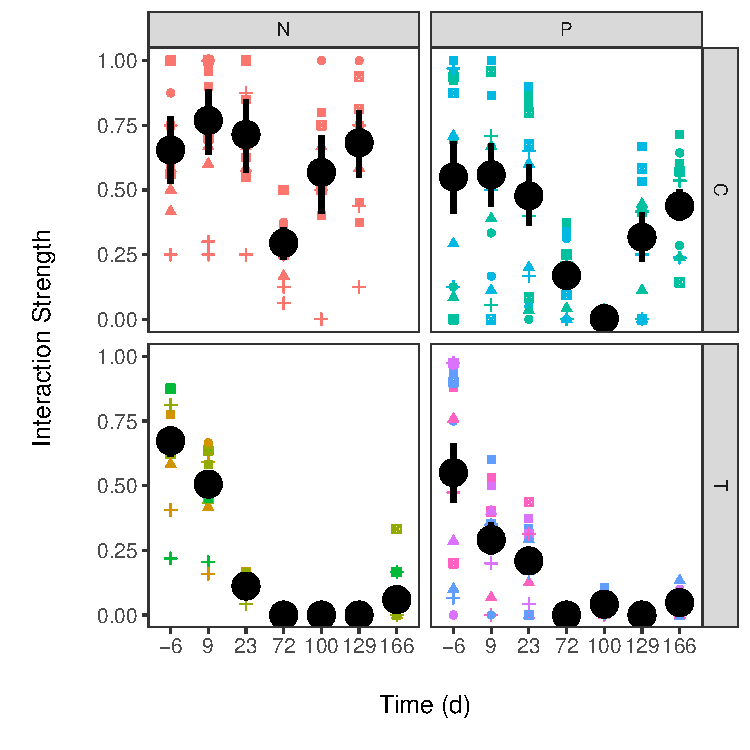
\includegraphics{analysis_ecoevostoich_files/figure-latex/unnamed-chunk-19-1.pdf}}{}}\label{section-1}

\begin{longtable}[]{@{}cccccc@{}}
\toprule
~ & Value & Std.Error & DF & t-value & p-value\tabularnewline
\midrule
\endhead
\textbf{(Intercept)} & 0.6579 & 0.04939 & 890 & 13.32 &
4.78e-37\tabularnewline
\bottomrule
\end{longtable}

\begin{verbatim}
    **trtT**          -0.2326     0.05573    5    -4.174   0.008707 

    **limP**          -0.2052     0.05857    5    -3.503    0.01723 

  **bac.time**       -0.0008318  0.0006544  890   -1.271     0.204  

 **trtT:limP**         0.1294     0.06874    5     1.882    0.1185  
\end{verbatim}

\textbf{trtT:bac.time} -0.002442 0.0007039 890 -3.469 0.0005475

\textbf{limP:bac.time} -0.0004828 0.0007306 890 -0.6608 0.5089

\subsection{\texorpdfstring{\textbf{trtT:limP:bac.time} 0.00113
0.0008153 890 1.386
0.1662}{trtT:limP:bac.time 0.00113 0.0008153 890 1.386 0.1662}}\label{trttlimpbac.time-0.00113-0.0008153-890-1.386-0.1662}

\begin{longtable}[]{@{}ccccc@{}}
\caption{Fixed effects: inf.prob \textasciitilde{} trt * lim *
bac.time}\tabularnewline
\toprule
\begin{minipage}[b]{0.08\columnwidth}\centering\strut
Min\strut
\end{minipage} & \begin{minipage}[b]{0.10\columnwidth}\centering\strut
Q1\strut
\end{minipage} & \begin{minipage}[b]{0.11\columnwidth}\centering\strut
Med\strut
\end{minipage} & \begin{minipage}[b]{0.08\columnwidth}\centering\strut
Q3\strut
\end{minipage} & \begin{minipage}[b]{0.08\columnwidth}\centering\strut
Max\strut
\end{minipage}\tabularnewline
\midrule
\endfirsthead
\toprule
\begin{minipage}[b]{0.08\columnwidth}\centering\strut
Min\strut
\end{minipage} & \begin{minipage}[b]{0.10\columnwidth}\centering\strut
Q1\strut
\end{minipage} & \begin{minipage}[b]{0.11\columnwidth}\centering\strut
Med\strut
\end{minipage} & \begin{minipage}[b]{0.08\columnwidth}\centering\strut
Q3\strut
\end{minipage} & \begin{minipage}[b]{0.08\columnwidth}\centering\strut
Max\strut
\end{minipage}\tabularnewline
\midrule
\endhead
\begin{minipage}[t]{0.08\columnwidth}\centering\strut
-2.338\strut
\end{minipage} & \begin{minipage}[t]{0.10\columnwidth}\centering\strut
-0.7711\strut
\end{minipage} & \begin{minipage}[t]{0.11\columnwidth}\centering\strut
-0.04333\strut
\end{minipage} & \begin{minipage}[t]{0.08\columnwidth}\centering\strut
0.6038\strut
\end{minipage} & \begin{minipage}[t]{0.08\columnwidth}\centering\strut
2.481\strut
\end{minipage}\tabularnewline
\bottomrule
\end{longtable}

\begin{longtable}[]{@{}cccc@{}}
\caption{Standardized Within-Group Residuals}\tabularnewline
\toprule
\begin{minipage}[b]{0.14\columnwidth}\centering\strut
~\strut
\end{minipage} & \begin{minipage}[b]{0.18\columnwidth}\centering\strut
Observations\strut
\end{minipage} & \begin{minipage}[b]{0.11\columnwidth}\centering\strut
Groups\strut
\end{minipage} & \begin{minipage}[b]{0.33\columnwidth}\centering\strut
Log-restricted-likelihood\strut
\end{minipage}\tabularnewline
\midrule
\endfirsthead
\toprule
\begin{minipage}[b]{0.14\columnwidth}\centering\strut
~\strut
\end{minipage} & \begin{minipage}[b]{0.18\columnwidth}\centering\strut
Observations\strut
\end{minipage} & \begin{minipage}[b]{0.11\columnwidth}\centering\strut
Groups\strut
\end{minipage} & \begin{minipage}[b]{0.33\columnwidth}\centering\strut
Log-restricted-likelihood\strut
\end{minipage}\tabularnewline
\midrule
\endhead
\begin{minipage}[t]{0.14\columnwidth}\centering\strut
\textbf{BcID}\strut
\end{minipage} & \begin{minipage}[t]{0.18\columnwidth}\centering\strut
903\strut
\end{minipage} & \begin{minipage}[t]{0.11\columnwidth}\centering\strut
9\strut
\end{minipage} & \begin{minipage}[t]{0.33\columnwidth}\centering\strut
-27.41\strut
\end{minipage}\tabularnewline
\bottomrule
\end{longtable}

\begin{longtable}[]{@{}cccccc@{}}
\caption{Linear mixed-effects model fit by REML : inf.prob
\textasciitilde{} trt * lim * bac.time}\tabularnewline
\toprule
\begin{minipage}[b]{0.23\columnwidth}\centering\strut
~\strut
\end{minipage} & \begin{minipage}[b]{0.12\columnwidth}\centering\strut
Value\strut
\end{minipage} & \begin{minipage}[b]{0.14\columnwidth}\centering\strut
Std.Error\strut
\end{minipage} & \begin{minipage}[b]{0.06\columnwidth}\centering\strut
DF\strut
\end{minipage} & \begin{minipage}[b]{0.12\columnwidth}\centering\strut
t-value\strut
\end{minipage} & \begin{minipage}[b]{0.12\columnwidth}\centering\strut
p-value\strut
\end{minipage}\tabularnewline
\midrule
\endfirsthead
\toprule
\begin{minipage}[b]{0.23\columnwidth}\centering\strut
~\strut
\end{minipage} & \begin{minipage}[b]{0.12\columnwidth}\centering\strut
Value\strut
\end{minipage} & \begin{minipage}[b]{0.14\columnwidth}\centering\strut
Std.Error\strut
\end{minipage} & \begin{minipage}[b]{0.06\columnwidth}\centering\strut
DF\strut
\end{minipage} & \begin{minipage}[b]{0.12\columnwidth}\centering\strut
t-value\strut
\end{minipage} & \begin{minipage}[b]{0.12\columnwidth}\centering\strut
p-value\strut
\end{minipage}\tabularnewline
\midrule
\endhead
\begin{minipage}[t]{0.23\columnwidth}\centering\strut
\textbf{(Intercept)}\strut
\end{minipage} & \begin{minipage}[t]{0.12\columnwidth}\centering\strut
0.4273\strut
\end{minipage} & \begin{minipage}[t]{0.14\columnwidth}\centering\strut
0.02265\strut
\end{minipage} & \begin{minipage}[t]{0.06\columnwidth}\centering\strut
601\strut
\end{minipage} & \begin{minipage}[t]{0.12\columnwidth}\centering\strut
18.87\strut
\end{minipage} & \begin{minipage}[t]{0.12\columnwidth}\centering\strut
1.049e-62\strut
\end{minipage}\tabularnewline
\begin{minipage}[t]{0.23\columnwidth}\centering\strut
\textbf{limP}\strut
\end{minipage} & \begin{minipage}[t]{0.12\columnwidth}\centering\strut
-0.07481\strut
\end{minipage} & \begin{minipage}[t]{0.14\columnwidth}\centering\strut
0.03158\strut
\end{minipage} & \begin{minipage}[t]{0.06\columnwidth}\centering\strut
4\strut
\end{minipage} & \begin{minipage}[t]{0.12\columnwidth}\centering\strut
-2.369\strut
\end{minipage} & \begin{minipage}[t]{0.12\columnwidth}\centering\strut
0.07689\strut
\end{minipage}\tabularnewline
\begin{minipage}[t]{0.23\columnwidth}\centering\strut
\textbf{bac.time}\strut
\end{minipage} & \begin{minipage}[t]{0.12\columnwidth}\centering\strut
-0.003292\strut
\end{minipage} & \begin{minipage}[t]{0.14\columnwidth}\centering\strut
0.0002187\strut
\end{minipage} & \begin{minipage}[t]{0.06\columnwidth}\centering\strut
601\strut
\end{minipage} & \begin{minipage}[t]{0.12\columnwidth}\centering\strut
-15.05\strut
\end{minipage} & \begin{minipage}[t]{0.12\columnwidth}\centering\strut
1.135e-43\strut
\end{minipage}\tabularnewline
\begin{minipage}[t]{0.23\columnwidth}\centering\strut
\textbf{limP:bac.time}\strut
\end{minipage} & \begin{minipage}[t]{0.12\columnwidth}\centering\strut
0.0006311\strut
\end{minipage} & \begin{minipage}[t]{0.14\columnwidth}\centering\strut
0.0003058\strut
\end{minipage} & \begin{minipage}[t]{0.06\columnwidth}\centering\strut
601\strut
\end{minipage} & \begin{minipage}[t]{0.12\columnwidth}\centering\strut
2.064\strut
\end{minipage} & \begin{minipage}[t]{0.12\columnwidth}\centering\strut
0.03943\strut
\end{minipage}\tabularnewline
\bottomrule
\end{longtable}

\begin{longtable}[]{@{}ccccc@{}}
\caption{Fixed effects: inf.prob \textasciitilde{} lim *
bac.time}\tabularnewline
\toprule
\begin{minipage}[b]{0.08\columnwidth}\centering\strut
Min\strut
\end{minipage} & \begin{minipage}[b]{0.10\columnwidth}\centering\strut
Q1\strut
\end{minipage} & \begin{minipage}[b]{0.11\columnwidth}\centering\strut
Med\strut
\end{minipage} & \begin{minipage}[b]{0.07\columnwidth}\centering\strut
Q3\strut
\end{minipage} & \begin{minipage}[b]{0.07\columnwidth}\centering\strut
Max\strut
\end{minipage}\tabularnewline
\midrule
\endfirsthead
\toprule
\begin{minipage}[b]{0.08\columnwidth}\centering\strut
Min\strut
\end{minipage} & \begin{minipage}[b]{0.10\columnwidth}\centering\strut
Q1\strut
\end{minipage} & \begin{minipage}[b]{0.11\columnwidth}\centering\strut
Med\strut
\end{minipage} & \begin{minipage}[b]{0.07\columnwidth}\centering\strut
Q3\strut
\end{minipage} & \begin{minipage}[b]{0.07\columnwidth}\centering\strut
Max\strut
\end{minipage}\tabularnewline
\midrule
\endhead
\begin{minipage}[t]{0.08\columnwidth}\centering\strut
-1.785\strut
\end{minipage} & \begin{minipage}[t]{0.10\columnwidth}\centering\strut
-0.7798\strut
\end{minipage} & \begin{minipage}[t]{0.11\columnwidth}\centering\strut
-0.04507\strut
\end{minipage} & \begin{minipage}[t]{0.07\columnwidth}\centering\strut
0.577\strut
\end{minipage} & \begin{minipage}[t]{0.07\columnwidth}\centering\strut
2.939\strut
\end{minipage}\tabularnewline
\bottomrule
\end{longtable}

\begin{longtable}[]{@{}cccc@{}}
\caption{Standardized Within-Group Residuals}\tabularnewline
\toprule
\begin{minipage}[b]{0.14\columnwidth}\centering\strut
~\strut
\end{minipage} & \begin{minipage}[b]{0.18\columnwidth}\centering\strut
Observations\strut
\end{minipage} & \begin{minipage}[b]{0.11\columnwidth}\centering\strut
Groups\strut
\end{minipage} & \begin{minipage}[b]{0.33\columnwidth}\centering\strut
Log-restricted-likelihood\strut
\end{minipage}\tabularnewline
\midrule
\endfirsthead
\toprule
\begin{minipage}[b]{0.14\columnwidth}\centering\strut
~\strut
\end{minipage} & \begin{minipage}[b]{0.18\columnwidth}\centering\strut
Observations\strut
\end{minipage} & \begin{minipage}[b]{0.11\columnwidth}\centering\strut
Groups\strut
\end{minipage} & \begin{minipage}[b]{0.33\columnwidth}\centering\strut
Log-restricted-likelihood\strut
\end{minipage}\tabularnewline
\midrule
\endhead
\begin{minipage}[t]{0.14\columnwidth}\centering\strut
\textbf{BcID}\strut
\end{minipage} & \begin{minipage}[t]{0.18\columnwidth}\centering\strut
609\strut
\end{minipage} & \begin{minipage}[t]{0.11\columnwidth}\centering\strut
6\strut
\end{minipage} & \begin{minipage}[t]{0.33\columnwidth}\centering\strut
102.8\strut
\end{minipage}\tabularnewline
\bottomrule
\end{longtable}

\begin{longtable}[]{@{}cccccc@{}}
\caption{Linear mixed-effects model fit by REML : inf.prob
\textasciitilde{} lim * bac.time}\tabularnewline
\toprule
\begin{minipage}[b]{0.23\columnwidth}\centering\strut
~\strut
\end{minipage} & \begin{minipage}[b]{0.13\columnwidth}\centering\strut
Value\strut
\end{minipage} & \begin{minipage}[b]{0.14\columnwidth}\centering\strut
Std.Error\strut
\end{minipage} & \begin{minipage}[b]{0.06\columnwidth}\centering\strut
DF\strut
\end{minipage} & \begin{minipage}[b]{0.12\columnwidth}\centering\strut
t-value\strut
\end{minipage} & \begin{minipage}[b]{0.12\columnwidth}\centering\strut
p-value\strut
\end{minipage}\tabularnewline
\midrule
\endfirsthead
\toprule
\begin{minipage}[b]{0.23\columnwidth}\centering\strut
~\strut
\end{minipage} & \begin{minipage}[b]{0.13\columnwidth}\centering\strut
Value\strut
\end{minipage} & \begin{minipage}[b]{0.14\columnwidth}\centering\strut
Std.Error\strut
\end{minipage} & \begin{minipage}[b]{0.06\columnwidth}\centering\strut
DF\strut
\end{minipage} & \begin{minipage}[b]{0.12\columnwidth}\centering\strut
t-value\strut
\end{minipage} & \begin{minipage}[b]{0.12\columnwidth}\centering\strut
p-value\strut
\end{minipage}\tabularnewline
\midrule
\endhead
\begin{minipage}[t]{0.23\columnwidth}\centering\strut
\textbf{(Intercept)}\strut
\end{minipage} & \begin{minipage}[t]{0.13\columnwidth}\centering\strut
0.661\strut
\end{minipage} & \begin{minipage}[t]{0.14\columnwidth}\centering\strut
0.06062\strut
\end{minipage} & \begin{minipage}[t]{0.06\columnwidth}\centering\strut
289\strut
\end{minipage} & \begin{minipage}[t]{0.12\columnwidth}\centering\strut
10.9\strut
\end{minipage} & \begin{minipage}[t]{0.12\columnwidth}\centering\strut
2.069e-23\strut
\end{minipage}\tabularnewline
\begin{minipage}[t]{0.23\columnwidth}\centering\strut
\textbf{limP}\strut
\end{minipage} & \begin{minipage}[t]{0.13\columnwidth}\centering\strut
-0.2057\strut
\end{minipage} & \begin{minipage}[t]{0.14\columnwidth}\centering\strut
0.072\strut
\end{minipage} & \begin{minipage}[t]{0.06\columnwidth}\centering\strut
1\strut
\end{minipage} & \begin{minipage}[t]{0.12\columnwidth}\centering\strut
-2.857\strut
\end{minipage} & \begin{minipage}[t]{0.12\columnwidth}\centering\strut
0.2143\strut
\end{minipage}\tabularnewline
\begin{minipage}[t]{0.23\columnwidth}\centering\strut
\textbf{bac.time}\strut
\end{minipage} & \begin{minipage}[t]{0.13\columnwidth}\centering\strut
-0.0008841\strut
\end{minipage} & \begin{minipage}[t]{0.14\columnwidth}\centering\strut
0.0008078\strut
\end{minipage} & \begin{minipage}[t]{0.06\columnwidth}\centering\strut
289\strut
\end{minipage} & \begin{minipage}[t]{0.12\columnwidth}\centering\strut
-1.094\strut
\end{minipage} & \begin{minipage}[t]{0.12\columnwidth}\centering\strut
0.2747\strut
\end{minipage}\tabularnewline
\begin{minipage}[t]{0.23\columnwidth}\centering\strut
\textbf{limP:bac.time}\strut
\end{minipage} & \begin{minipage}[t]{0.13\columnwidth}\centering\strut
-0.0004692\strut
\end{minipage} & \begin{minipage}[t]{0.14\columnwidth}\centering\strut
0.0009035\strut
\end{minipage} & \begin{minipage}[t]{0.06\columnwidth}\centering\strut
289\strut
\end{minipage} & \begin{minipage}[t]{0.12\columnwidth}\centering\strut
-0.5193\strut
\end{minipage} & \begin{minipage}[t]{0.12\columnwidth}\centering\strut
0.6039\strut
\end{minipage}\tabularnewline
\bottomrule
\end{longtable}

\begin{longtable}[]{@{}ccccc@{}}
\caption{Fixed effects: inf.prob \textasciitilde{} lim *
bac.time}\tabularnewline
\toprule
\begin{minipage}[b]{0.08\columnwidth}\centering\strut
Min\strut
\end{minipage} & \begin{minipage}[b]{0.08\columnwidth}\centering\strut
Q1\strut
\end{minipage} & \begin{minipage}[b]{0.11\columnwidth}\centering\strut
Med\strut
\end{minipage} & \begin{minipage}[b]{0.08\columnwidth}\centering\strut
Q3\strut
\end{minipage} & \begin{minipage}[b]{0.08\columnwidth}\centering\strut
Max\strut
\end{minipage}\tabularnewline
\midrule
\endfirsthead
\toprule
\begin{minipage}[b]{0.08\columnwidth}\centering\strut
Min\strut
\end{minipage} & \begin{minipage}[b]{0.08\columnwidth}\centering\strut
Q1\strut
\end{minipage} & \begin{minipage}[b]{0.11\columnwidth}\centering\strut
Med\strut
\end{minipage} & \begin{minipage}[b]{0.08\columnwidth}\centering\strut
Q3\strut
\end{minipage} & \begin{minipage}[b]{0.08\columnwidth}\centering\strut
Max\strut
\end{minipage}\tabularnewline
\midrule
\endhead
\begin{minipage}[t]{0.08\columnwidth}\centering\strut
-1.829\strut
\end{minipage} & \begin{minipage}[t]{0.08\columnwidth}\centering\strut
-1.022\strut
\end{minipage} & \begin{minipage}[t]{0.11\columnwidth}\centering\strut
-0.07812\strut
\end{minipage} & \begin{minipage}[t]{0.08\columnwidth}\centering\strut
0.8374\strut
\end{minipage} & \begin{minipage}[t]{0.08\columnwidth}\centering\strut
1.779\strut
\end{minipage}\tabularnewline
\bottomrule
\end{longtable}

\begin{longtable}[]{@{}cccc@{}}
\caption{Standardized Within-Group Residuals}\tabularnewline
\toprule
\begin{minipage}[b]{0.14\columnwidth}\centering\strut
~\strut
\end{minipage} & \begin{minipage}[b]{0.18\columnwidth}\centering\strut
Observations\strut
\end{minipage} & \begin{minipage}[b]{0.11\columnwidth}\centering\strut
Groups\strut
\end{minipage} & \begin{minipage}[b]{0.33\columnwidth}\centering\strut
Log-restricted-likelihood\strut
\end{minipage}\tabularnewline
\midrule
\endfirsthead
\toprule
\begin{minipage}[b]{0.14\columnwidth}\centering\strut
~\strut
\end{minipage} & \begin{minipage}[b]{0.18\columnwidth}\centering\strut
Observations\strut
\end{minipage} & \begin{minipage}[b]{0.11\columnwidth}\centering\strut
Groups\strut
\end{minipage} & \begin{minipage}[b]{0.33\columnwidth}\centering\strut
Log-restricted-likelihood\strut
\end{minipage}\tabularnewline
\midrule
\endhead
\begin{minipage}[t]{0.14\columnwidth}\centering\strut
\textbf{BcID}\strut
\end{minipage} & \begin{minipage}[t]{0.18\columnwidth}\centering\strut
294\strut
\end{minipage} & \begin{minipage}[t]{0.11\columnwidth}\centering\strut
3\strut
\end{minipage} & \begin{minipage}[t]{0.33\columnwidth}\centering\strut
-87.31\strut
\end{minipage}\tabularnewline
\bottomrule
\end{longtable}

Table: Linear mixed-effects model fit by REML : inf.prob
\textasciitilde{} lim * bac.time

\newpage

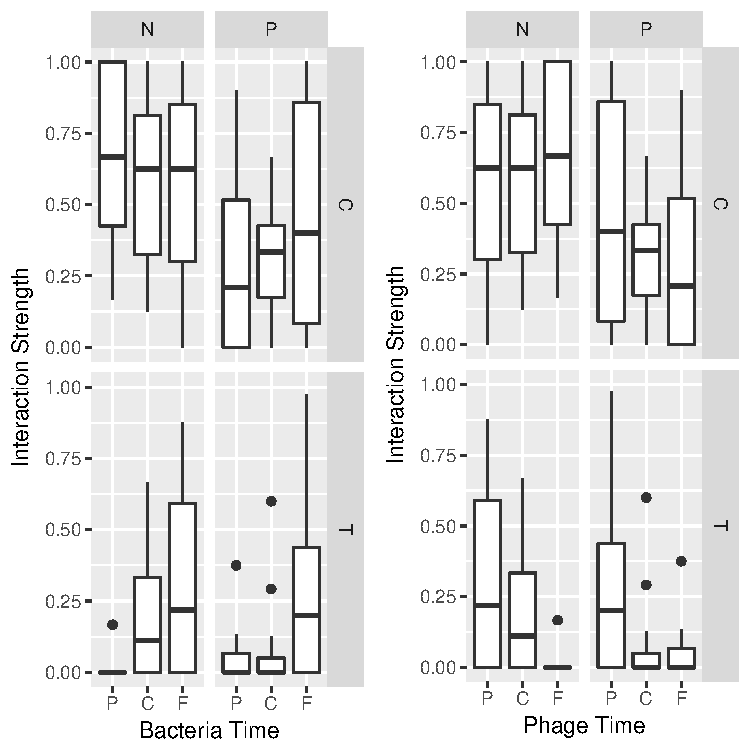
\includegraphics{analysis_ecoevostoich_files/figure-latex/unnamed-chunk-20-1.pdf}

\newpage

\subsection{RMANOVA for Interaction
Strengths}\label{rmanova-for-interaction-strengths}

\begin{longtable}[]{@{}cccccc@{}}
\toprule
\begin{minipage}[b]{0.21\columnwidth}\centering\strut
~\strut
\end{minipage} & \begin{minipage}[b]{0.07\columnwidth}\centering\strut
AIC\strut
\end{minipage} & \begin{minipage}[b]{0.07\columnwidth}\centering\strut
BIC\strut
\end{minipage} & \begin{minipage}[b]{0.10\columnwidth}\centering\strut
logLik\strut
\end{minipage} & \begin{minipage}[b]{0.12\columnwidth}\centering\strut
L.Ratio\strut
\end{minipage} & \begin{minipage}[b]{0.12\columnwidth}\centering\strut
p-value\strut
\end{minipage}\tabularnewline
\midrule
\endhead
\begin{minipage}[t]{0.21\columnwidth}\centering\strut
\textbf{model.ar}\strut
\end{minipage} & \begin{minipage}[t]{0.07\columnwidth}\centering\strut
169.1\strut
\end{minipage} & \begin{minipage}[t]{0.07\columnwidth}\centering\strut
260.1\strut
\end{minipage} & \begin{minipage}[t]{0.10\columnwidth}\centering\strut
-65.57\strut
\end{minipage} & \begin{minipage}[t]{0.12\columnwidth}\centering\strut
NA\strut
\end{minipage} & \begin{minipage}[t]{0.12\columnwidth}\centering\strut
NA\strut
\end{minipage}\tabularnewline
\begin{minipage}[t]{0.21\columnwidth}\centering\strut
\textbf{model.arma1}\strut
\end{minipage} & \begin{minipage}[t]{0.07\columnwidth}\centering\strut
115.5\strut
\end{minipage} & \begin{minipage}[t]{0.07\columnwidth}\centering\strut
211.3\strut
\end{minipage} & \begin{minipage}[t]{0.10\columnwidth}\centering\strut
-37.76\strut
\end{minipage} & \begin{minipage}[t]{0.12\columnwidth}\centering\strut
55.63\strut
\end{minipage} & \begin{minipage}[t]{0.12\columnwidth}\centering\strut
8.769e-14\strut
\end{minipage}\tabularnewline
\begin{minipage}[t]{0.21\columnwidth}\centering\strut
\textbf{model.arma2}\strut
\end{minipage} & \begin{minipage}[t]{0.07\columnwidth}\centering\strut
98.61\strut
\end{minipage} & \begin{minipage}[t]{0.07\columnwidth}\centering\strut
199.2\strut
\end{minipage} & \begin{minipage}[t]{0.10\columnwidth}\centering\strut
-28.31\strut
\end{minipage} & \begin{minipage}[t]{0.12\columnwidth}\centering\strut
18.91\strut
\end{minipage} & \begin{minipage}[t]{0.12\columnwidth}\centering\strut
1.37e-05\strut
\end{minipage}\tabularnewline
\bottomrule
\end{longtable}

\begin{longtable}[]{@{}llll@{}}
\toprule
\begin{minipage}[b]{0.43\columnwidth}\raggedright\strut
~\strut
\end{minipage} & \begin{minipage}[b]{0.17\columnwidth}\raggedright\strut
Std.Error\strut
\end{minipage} & \begin{minipage}[b]{0.13\columnwidth}\raggedright\strut
t-value\strut
\end{minipage} & \begin{minipage}[b]{0.16\columnwidth}\raggedright\strut
p-value\strut
\end{minipage}\tabularnewline
\midrule
\endhead
\begin{minipage}[t]{0.43\columnwidth}\raggedright\strut
\textbf{(Intercept)}\strut
\end{minipage} & \begin{minipage}[t]{0.17\columnwidth}\raggedright\strut
\textbf{0.07713}\strut
\end{minipage} & \begin{minipage}[t]{0.13\columnwidth}\raggedright\strut
\textbf{9.872}\strut
\end{minipage} & \begin{minipage}[t]{0.16\columnwidth}\raggedright\strut
\textbf{7.099e-22}\strut
\end{minipage}\tabularnewline
\begin{minipage}[t]{0.43\columnwidth}\raggedright\strut
\textbf{trtT}\strut
\end{minipage} & \begin{minipage}[t]{0.17\columnwidth}\raggedright\strut
\textbf{0.08638}\strut
\end{minipage} & \begin{minipage}[t]{0.13\columnwidth}\raggedright\strut
\textbf{-3.702}\strut
\end{minipage} & \begin{minipage}[t]{0.16\columnwidth}\raggedright\strut
\textbf{0.0002276}\strut
\end{minipage}\tabularnewline
\begin{minipage}[t]{0.43\columnwidth}\raggedright\strut
\textbf{limP}\strut
\end{minipage} & \begin{minipage}[t]{0.17\columnwidth}\raggedright\strut
\textbf{0.09298}\strut
\end{minipage} & \begin{minipage}[t]{0.13\columnwidth}\raggedright\strut
\textbf{-4.93}\strut
\end{minipage} & \begin{minipage}[t]{0.16\columnwidth}\raggedright\strut
\textbf{0.007875}\strut
\end{minipage}\tabularnewline
\begin{minipage}[t]{0.43\columnwidth}\raggedright\strut
\textbf{phage.time}\strut
\end{minipage} & \begin{minipage}[t]{0.17\columnwidth}\raggedright\strut
0.0006172\strut
\end{minipage} & \begin{minipage}[t]{0.13\columnwidth}\raggedright\strut
-1.916\strut
\end{minipage} & \begin{minipage}[t]{0.16\columnwidth}\raggedright\strut
0.05569\strut
\end{minipage}\tabularnewline
\begin{minipage}[t]{0.43\columnwidth}\raggedright\strut
\textbf{bac.time}\strut
\end{minipage} & \begin{minipage}[t]{0.17\columnwidth}\raggedright\strut
0.001005\strut
\end{minipage} & \begin{minipage}[t]{0.13\columnwidth}\raggedright\strut
0.1231\strut
\end{minipage} & \begin{minipage}[t]{0.16\columnwidth}\raggedright\strut
0.9021\strut
\end{minipage}\tabularnewline
\begin{minipage}[t]{0.43\columnwidth}\raggedright\strut
\textbf{trtT:limP}\strut
\end{minipage} & \begin{minipage}[t]{0.17\columnwidth}\raggedright\strut
0.1078\strut
\end{minipage} & \begin{minipage}[t]{0.13\columnwidth}\raggedright\strut
1.856\strut
\end{minipage} & \begin{minipage}[t]{0.16\columnwidth}\raggedright\strut
0.06381\strut
\end{minipage}\tabularnewline
\begin{minipage}[t]{0.43\columnwidth}\raggedright\strut
\textbf{trtT:phage.time}\strut
\end{minipage} & \begin{minipage}[t]{0.17\columnwidth}\raggedright\strut
0.0007027\strut
\end{minipage} & \begin{minipage}[t]{0.13\columnwidth}\raggedright\strut
1.008\strut
\end{minipage} & \begin{minipage}[t]{0.16\columnwidth}\raggedright\strut
0.3136\strut
\end{minipage}\tabularnewline
\begin{minipage}[t]{0.43\columnwidth}\raggedright\strut
\textbf{limP:phage.time}\strut
\end{minipage} & \begin{minipage}[t]{0.17\columnwidth}\raggedright\strut
\textbf{0.0007399}\strut
\end{minipage} & \begin{minipage}[t]{0.13\columnwidth}\raggedright\strut
\textbf{3.511}\strut
\end{minipage} & \begin{minipage}[t]{0.16\columnwidth}\raggedright\strut
\textbf{0.0004695}\strut
\end{minipage}\tabularnewline
\begin{minipage}[t]{0.43\columnwidth}\raggedright\strut
\textbf{trtT:bac.time}\strut
\end{minipage} & \begin{minipage}[t]{0.17\columnwidth}\raggedright\strut
\textbf{0.001097}\strut
\end{minipage} & \begin{minipage}[t]{0.13\columnwidth}\raggedright\strut
\textbf{-3.091}\strut
\end{minipage} & \begin{minipage}[t]{0.16\columnwidth}\raggedright\strut
\textbf{0.00206}\strut
\end{minipage}\tabularnewline
\begin{minipage}[t]{0.43\columnwidth}\raggedright\strut
\textbf{limP:bac.time}\strut
\end{minipage} & \begin{minipage}[t]{0.17\columnwidth}\raggedright\strut
0.001136\strut
\end{minipage} & \begin{minipage}[t]{0.13\columnwidth}\raggedright\strut
-0.02436\strut
\end{minipage} & \begin{minipage}[t]{0.16\columnwidth}\raggedright\strut
0.9806\strut
\end{minipage}\tabularnewline
\begin{minipage}[t]{0.43\columnwidth}\raggedright\strut
\textbf{phage.time:bac.time}\strut
\end{minipage} & \begin{minipage}[t]{0.17\columnwidth}\raggedright\strut
8.462e-06\strut
\end{minipage} & \begin{minipage}[t]{0.13\columnwidth}\raggedright\strut
-1.811\strut
\end{minipage} & \begin{minipage}[t]{0.16\columnwidth}\raggedright\strut
0.07056\strut
\end{minipage}\tabularnewline
\begin{minipage}[t]{0.43\columnwidth}\raggedright\strut
\textbf{trtT:limP:phage.time}\strut
\end{minipage} & \begin{minipage}[t]{0.17\columnwidth}\raggedright\strut
0.0008774\strut
\end{minipage} & \begin{minipage}[t]{0.13\columnwidth}\raggedright\strut
-0.9831\strut
\end{minipage} & \begin{minipage}[t]{0.16\columnwidth}\raggedright\strut
0.3258\strut
\end{minipage}\tabularnewline
\begin{minipage}[t]{0.43\columnwidth}\raggedright\strut
\textbf{trtT:limP:bac.time}\strut
\end{minipage} & \begin{minipage}[t]{0.17\columnwidth}\raggedright\strut
0.001294\strut
\end{minipage} & \begin{minipage}[t]{0.13\columnwidth}\raggedright\strut
1.933\strut
\end{minipage} & \begin{minipage}[t]{0.16\columnwidth}\raggedright\strut
0.05351\strut
\end{minipage}\tabularnewline
\begin{minipage}[t]{0.43\columnwidth}\raggedright\strut
\textbf{trtT:phage.time:bac.time}\strut
\end{minipage} & \begin{minipage}[t]{0.17\columnwidth}\raggedright\strut
\textbf{9.205e-06}\strut
\end{minipage} & \begin{minipage}[t]{0.13\columnwidth}\raggedright\strut
\textbf{2.014}\strut
\end{minipage} & \begin{minipage}[t]{0.16\columnwidth}\raggedright\strut
\textbf{0.04427}\strut
\end{minipage}\tabularnewline
\begin{minipage}[t]{0.43\columnwidth}\raggedright\strut
\textbf{limP:phage.time:bac.time}\strut
\end{minipage} & \begin{minipage}[t]{0.17\columnwidth}\raggedright\strut
9.576e-06\strut
\end{minipage} & \begin{minipage}[t]{0.13\columnwidth}\raggedright\strut
0.4493\strut
\end{minipage} & \begin{minipage}[t]{0.16\columnwidth}\raggedright\strut
0.6533\strut
\end{minipage}\tabularnewline
\begin{minipage}[t]{0.43\columnwidth}\raggedright\strut
\textbf{trtT:limP:phage.time:bac.time}\strut
\end{minipage} & \begin{minipage}[t]{0.17\columnwidth}\raggedright\strut
1.086e-05\strut
\end{minipage} & \begin{minipage}[t]{0.13\columnwidth}\raggedright\strut
-1.801\strut
\end{minipage} & \begin{minipage}[t]{0.16\columnwidth}\raggedright\strut
0.07197\strut
\end{minipage}\tabularnewline
\bottomrule
\end{longtable}

\newpage

\subsection{Infection dynamics by
chemostat}\label{infection-dynamics-by-chemostat}

\newpage

\subsection{Infection dynamics by
treatment}\label{infection-dynamics-by-treatment}

\subsubsection{Network plots}\label{network-plots}

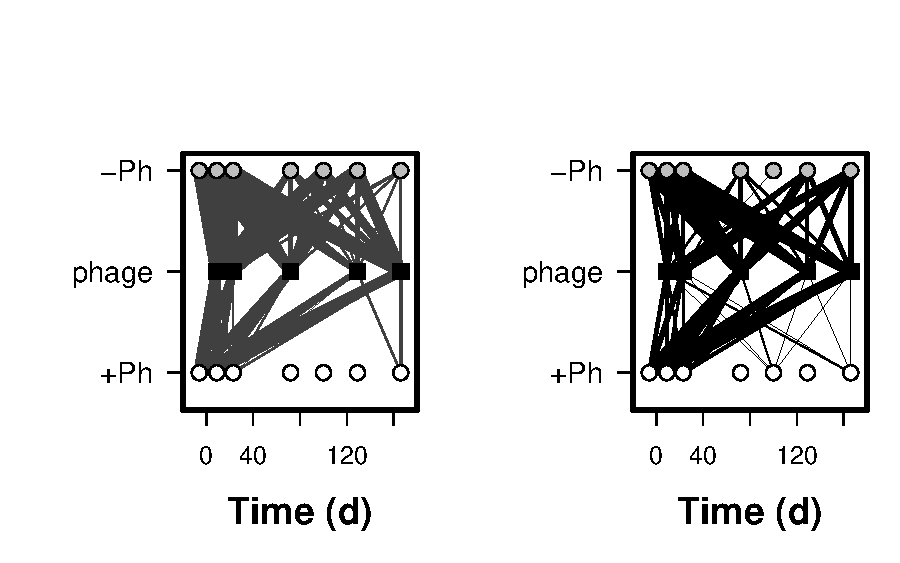
\includegraphics{analysis_ecoevostoich_files/figure-latex/coevo-pub/fig-1.pdf}

\begin{verbatim}
## null device 
##           1
\end{verbatim}

\newpage

\subsection{Community Networks}\label{community-networks}

\newpage

\subsection{BiWeb estimates for nestedness and
modularity}\label{biweb-estimates-for-nestedness-and-modularity}

\begin{longtable}[]{@{}cccc@{}}
\toprule
\begin{minipage}[b]{0.24\columnwidth}\centering\strut
~\strut
\end{minipage} & \begin{minipage}[b]{0.23\columnwidth}\centering\strut
statistic.t\strut
\end{minipage} & \begin{minipage}[b]{0.20\columnwidth}\centering\strut
parameter.df\strut
\end{minipage} & \begin{minipage}[b]{0.22\columnwidth}\centering\strut
p.value\strut
\end{minipage}\tabularnewline
\midrule
\endhead
\begin{minipage}[t]{0.24\columnwidth}\centering\strut
\textbf{connectance}\strut
\end{minipage} & \begin{minipage}[t]{0.23\columnwidth}\centering\strut
1.456400410208\strut
\end{minipage} & \begin{minipage}[t]{0.20\columnwidth}\centering\strut
3.89610299683149\strut
\end{minipage} & \begin{minipage}[t]{0.22\columnwidth}\centering\strut
0.220826873899216\strut
\end{minipage}\tabularnewline
\begin{minipage}[t]{0.24\columnwidth}\centering\strut
\textbf{modularity.qb}\strut
\end{minipage} & \begin{minipage}[t]{0.23\columnwidth}\centering\strut
-3.5488938188692\strut
\end{minipage} & \begin{minipage}[t]{0.20\columnwidth}\centering\strut
3.00184431086153\strut
\end{minipage} & \begin{minipage}[t]{0.22\columnwidth}\centering\strut
0.0380832752236465\strut
\end{minipage}\tabularnewline
\begin{minipage}[t]{0.24\columnwidth}\centering\strut
\textbf{modularity.qr}\strut
\end{minipage} & \begin{minipage}[t]{0.23\columnwidth}\centering\strut
-0.337865126206578\strut
\end{minipage} & \begin{minipage}[t]{0.20\columnwidth}\centering\strut
3.62274149633006\strut
\end{minipage} & \begin{minipage}[t]{0.22\columnwidth}\centering\strut
0.754122338605035\strut
\end{minipage}\tabularnewline
\begin{minipage}[t]{0.24\columnwidth}\centering\strut
\textbf{nodf}\strut
\end{minipage} & \begin{minipage}[t]{0.23\columnwidth}\centering\strut
0.371973397721244\strut
\end{minipage} & \begin{minipage}[t]{0.20\columnwidth}\centering\strut
3.80924523421393\strut
\end{minipage} & \begin{minipage}[t]{0.22\columnwidth}\centering\strut
0.729674513225951\strut
\end{minipage}\tabularnewline
\begin{minipage}[t]{0.24\columnwidth}\centering\strut
\textbf{ntc}\strut
\end{minipage} & \begin{minipage}[t]{0.23\columnwidth}\centering\strut
-0.848020202172062\strut
\end{minipage} & \begin{minipage}[t]{0.20\columnwidth}\centering\strut
3.96441380258424\strut
\end{minipage} & \begin{minipage}[t]{0.22\columnwidth}\centering\strut
0.444591439999469\strut
\end{minipage}\tabularnewline
\bottomrule
\end{longtable}

\newpage

\subsection{\texorpdfstring{\textbf{Synechococcus}
resistance}{Synechococcus resistance}}\label{synechococcus-resistance}

\subsubsection{global; sympatric vs.~allopatric
resistance}\label{global-sympatric-vs.allopatric-resistance}

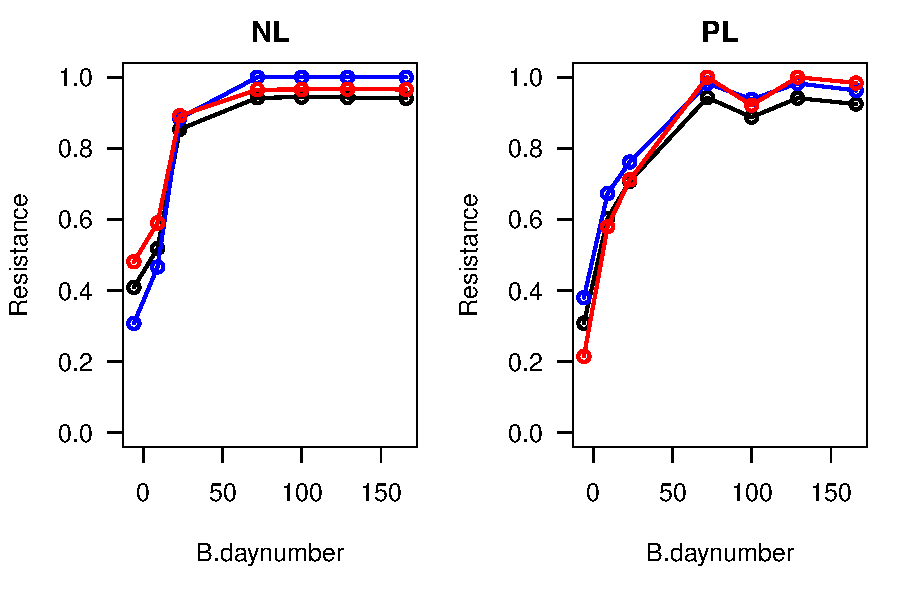
\includegraphics{analysis_ecoevostoich_files/figure-latex/unnamed-chunk-30-1.pdf}

\begin{verbatim}
##                   numDF denDF  F-value p-value
## (Intercept)           1    97 43.84393  <.0001
## B.trt                 1     4  1.45906  0.2936
## B.daynumber           6    97 14.27125  <.0001
## B.trt:B.daynumber     6    97  0.51041  0.7992
\end{verbatim}

\begin{longtable}[]{@{}ccccc@{}}
\toprule
\begin{minipage}[b]{0.29\columnwidth}\centering\strut
~\strut
\end{minipage} & \begin{minipage}[b]{0.10\columnwidth}\centering\strut
numDF\strut
\end{minipage} & \begin{minipage}[b]{0.10\columnwidth}\centering\strut
denDF\strut
\end{minipage} & \begin{minipage}[b]{0.12\columnwidth}\centering\strut
F-value\strut
\end{minipage} & \begin{minipage}[b]{0.12\columnwidth}\centering\strut
p-value\strut
\end{minipage}\tabularnewline
\midrule
\endhead
\begin{minipage}[t]{0.29\columnwidth}\centering\strut
\textbf{(Intercept)}\strut
\end{minipage} & \begin{minipage}[t]{0.10\columnwidth}\centering\strut
1\strut
\end{minipage} & \begin{minipage}[t]{0.10\columnwidth}\centering\strut
97\strut
\end{minipage} & \begin{minipage}[t]{0.12\columnwidth}\centering\strut
2184\strut
\end{minipage} & \begin{minipage}[t]{0.12\columnwidth}\centering\strut
0\strut
\end{minipage}\tabularnewline
\begin{minipage}[t]{0.29\columnwidth}\centering\strut
\textbf{B.trt}\strut
\end{minipage} & \begin{minipage}[t]{0.10\columnwidth}\centering\strut
1\strut
\end{minipage} & \begin{minipage}[t]{0.10\columnwidth}\centering\strut
4\strut
\end{minipage} & \begin{minipage}[t]{0.12\columnwidth}\centering\strut
0.05589\strut
\end{minipage} & \begin{minipage}[t]{0.12\columnwidth}\centering\strut
0.8247\strut
\end{minipage}\tabularnewline
\begin{minipage}[t]{0.29\columnwidth}\centering\strut
\textbf{B.daynumber}\strut
\end{minipage} & \begin{minipage}[t]{0.10\columnwidth}\centering\strut
6\strut
\end{minipage} & \begin{minipage}[t]{0.10\columnwidth}\centering\strut
97\strut
\end{minipage} & \begin{minipage}[t]{0.12\columnwidth}\centering\strut
31.82\strut
\end{minipage} & \begin{minipage}[t]{0.12\columnwidth}\centering\strut
0\strut
\end{minipage}\tabularnewline
\begin{minipage}[t]{0.29\columnwidth}\centering\strut
\textbf{B.trt:B.daynumber}\strut
\end{minipage} & \begin{minipage}[t]{0.10\columnwidth}\centering\strut
6\strut
\end{minipage} & \begin{minipage}[t]{0.10\columnwidth}\centering\strut
97\strut
\end{minipage} & \begin{minipage}[t]{0.12\columnwidth}\centering\strut
0.5104\strut
\end{minipage} & \begin{minipage}[t]{0.12\columnwidth}\centering\strut
0.7992\strut
\end{minipage}\tabularnewline
\bottomrule
\end{longtable}

\begin{longtable}[]{@{}ccccc@{}}
\toprule
\begin{minipage}[b]{0.29\columnwidth}\centering\strut
~\strut
\end{minipage} & \begin{minipage}[b]{0.10\columnwidth}\centering\strut
numDF\strut
\end{minipage} & \begin{minipage}[b]{0.10\columnwidth}\centering\strut
denDF\strut
\end{minipage} & \begin{minipage}[b]{0.12\columnwidth}\centering\strut
F-value\strut
\end{minipage} & \begin{minipage}[b]{0.12\columnwidth}\centering\strut
p-value\strut
\end{minipage}\tabularnewline
\midrule
\endhead
\begin{minipage}[t]{0.29\columnwidth}\centering\strut
\textbf{(Intercept)}\strut
\end{minipage} & \begin{minipage}[t]{0.10\columnwidth}\centering\strut
1\strut
\end{minipage} & \begin{minipage}[t]{0.10\columnwidth}\centering\strut
97\strut
\end{minipage} & \begin{minipage}[t]{0.12\columnwidth}\centering\strut
1645\strut
\end{minipage} & \begin{minipage}[t]{0.12\columnwidth}\centering\strut
0\strut
\end{minipage}\tabularnewline
\begin{minipage}[t]{0.29\columnwidth}\centering\strut
\textbf{B.trt}\strut
\end{minipage} & \begin{minipage}[t]{0.10\columnwidth}\centering\strut
1\strut
\end{minipage} & \begin{minipage}[t]{0.10\columnwidth}\centering\strut
4\strut
\end{minipage} & \begin{minipage}[t]{0.12\columnwidth}\centering\strut
1.962\strut
\end{minipage} & \begin{minipage}[t]{0.12\columnwidth}\centering\strut
0.2339\strut
\end{minipage}\tabularnewline
\begin{minipage}[t]{0.29\columnwidth}\centering\strut
\textbf{B.daynumber}\strut
\end{minipage} & \begin{minipage}[t]{0.10\columnwidth}\centering\strut
6\strut
\end{minipage} & \begin{minipage}[t]{0.10\columnwidth}\centering\strut
97\strut
\end{minipage} & \begin{minipage}[t]{0.12\columnwidth}\centering\strut
27.78\strut
\end{minipage} & \begin{minipage}[t]{0.12\columnwidth}\centering\strut
0\strut
\end{minipage}\tabularnewline
\begin{minipage}[t]{0.29\columnwidth}\centering\strut
\textbf{B.trt:B.daynumber}\strut
\end{minipage} & \begin{minipage}[t]{0.10\columnwidth}\centering\strut
6\strut
\end{minipage} & \begin{minipage}[t]{0.10\columnwidth}\centering\strut
97\strut
\end{minipage} & \begin{minipage}[t]{0.12\columnwidth}\centering\strut
0.7992\strut
\end{minipage} & \begin{minipage}[t]{0.12\columnwidth}\centering\strut
0.5729\strut
\end{minipage}\tabularnewline
\bottomrule
\end{longtable}

\begin{longtable}[]{@{}ccccc@{}}
\toprule
\begin{minipage}[b]{0.29\columnwidth}\centering\strut
~\strut
\end{minipage} & \begin{minipage}[b]{0.10\columnwidth}\centering\strut
numDF\strut
\end{minipage} & \begin{minipage}[b]{0.10\columnwidth}\centering\strut
denDF\strut
\end{minipage} & \begin{minipage}[b]{0.12\columnwidth}\centering\strut
F-value\strut
\end{minipage} & \begin{minipage}[b]{0.12\columnwidth}\centering\strut
p-value\strut
\end{minipage}\tabularnewline
\midrule
\endhead
\begin{minipage}[t]{0.29\columnwidth}\centering\strut
\textbf{(Intercept)}\strut
\end{minipage} & \begin{minipage}[t]{0.10\columnwidth}\centering\strut
1\strut
\end{minipage} & \begin{minipage}[t]{0.10\columnwidth}\centering\strut
97\strut
\end{minipage} & \begin{minipage}[t]{0.12\columnwidth}\centering\strut
2394\strut
\end{minipage} & \begin{minipage}[t]{0.12\columnwidth}\centering\strut
0\strut
\end{minipage}\tabularnewline
\begin{minipage}[t]{0.29\columnwidth}\centering\strut
\textbf{B.trt}\strut
\end{minipage} & \begin{minipage}[t]{0.10\columnwidth}\centering\strut
1\strut
\end{minipage} & \begin{minipage}[t]{0.10\columnwidth}\centering\strut
4\strut
\end{minipage} & \begin{minipage}[t]{0.12\columnwidth}\centering\strut
0.4009\strut
\end{minipage} & \begin{minipage}[t]{0.12\columnwidth}\centering\strut
0.561\strut
\end{minipage}\tabularnewline
\begin{minipage}[t]{0.29\columnwidth}\centering\strut
\textbf{B.daynumber}\strut
\end{minipage} & \begin{minipage}[t]{0.10\columnwidth}\centering\strut
6\strut
\end{minipage} & \begin{minipage}[t]{0.10\columnwidth}\centering\strut
97\strut
\end{minipage} & \begin{minipage}[t]{0.12\columnwidth}\centering\strut
36.72\strut
\end{minipage} & \begin{minipage}[t]{0.12\columnwidth}\centering\strut
0\strut
\end{minipage}\tabularnewline
\begin{minipage}[t]{0.29\columnwidth}\centering\strut
\textbf{B.trt:B.daynumber}\strut
\end{minipage} & \begin{minipage}[t]{0.10\columnwidth}\centering\strut
6\strut
\end{minipage} & \begin{minipage}[t]{0.10\columnwidth}\centering\strut
97\strut
\end{minipage} & \begin{minipage}[t]{0.12\columnwidth}\centering\strut
1.557\strut
\end{minipage} & \begin{minipage}[t]{0.12\columnwidth}\centering\strut
0.168\strut
\end{minipage}\tabularnewline
\bottomrule
\end{longtable}

\newpage

\subsubsection{Compositional resistance}\label{compositional-resistance}

\subsection{\texorpdfstring{\protect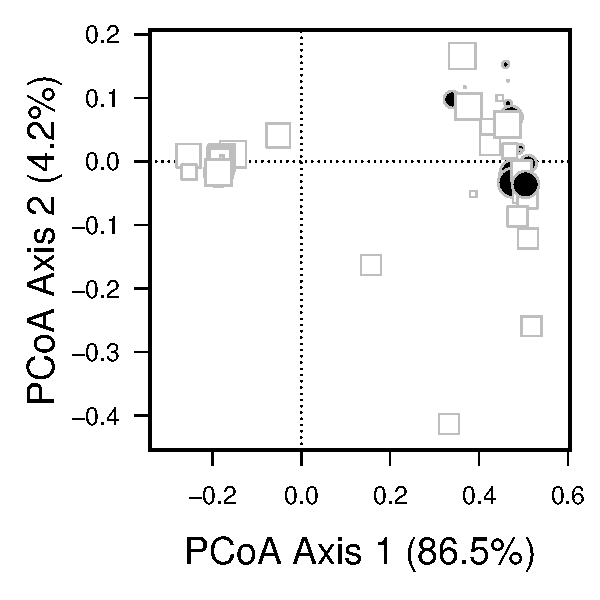
\includegraphics{analysis_ecoevostoich_files/figure-latex/unnamed-chunk-32-1.pdf}}{}}\label{section-2}

\begin{longtable}[]{@{}ccccccc@{}}
\toprule
~ & Df & SumsOfSqs & MeanSqs & F.Model & R2 &
Pr(\textgreater{}F)\tabularnewline
\midrule
\endhead
\textbf{Time} & 1 & 4.242 & 4.242 & 71.5 & 0.39 & 0.001\tabularnewline
\bottomrule
\end{longtable}

\textbf{Limitation} 1 0.03804 0.03804 0.6411 0.003496 0.017

**Time*Limitation** 1 0.07149 0.07149 1.205 0.006572 0.258

\begin{verbatim}
**Residuals**     110     6.527     0.05933     NA       0.6       NA   

  **Total**       113     10.88       NA        NA        1        NA   
\end{verbatim}

\begin{center}\rule{0.5\linewidth}{\linethickness}\end{center}

Table: Blocks: strata

\newpage

\subsection{Phage Host Range}\label{phage-host-range}

\subsubsection{global; sympatric vs.~allopatric host
range}\label{global-sympatric-vs.allopatric-host-range}

\newpage

\subsubsection{Compositional
infectivity}\label{compositional-infectivity}

\newpage

\subsection{Treatement level degree of
infection}\label{treatement-level-degree-of-infection}

\newpage

\section{Appendix}\label{appendix}

\subsection{R and packages}\label{r-and-packages}

All analyses were completed using R version 3.3.2 (2016-10-31)

\newpage

\subsection{References}\label{references}

\newpage

\subsection{Appendix}\label{appendix-1}

\subsubsection{Key term definitions}\label{key-term-definitions}

\begin{longtable}[]{@{}ccc@{}}
\toprule
\begin{minipage}[b]{0.24\columnwidth}\centering\strut
Word\strut
\end{minipage} & \begin{minipage}[b]{0.19\columnwidth}\centering\strut
Abbreviation\strut
\end{minipage} & \begin{minipage}[b]{0.15\columnwidth}\centering\strut
Definition\strut
\end{minipage}\tabularnewline
\midrule
\endhead
\begin{minipage}[t]{0.24\columnwidth}\centering\strut
Nitrogen\strut
\end{minipage} & \begin{minipage}[t]{0.19\columnwidth}\centering\strut
N\strut
\end{minipage} & \begin{minipage}[t]{0.15\columnwidth}\centering\strut
\strut
\end{minipage}\tabularnewline
\begin{minipage}[t]{0.24\columnwidth}\centering\strut
Phosphorus\strut
\end{minipage} & \begin{minipage}[t]{0.19\columnwidth}\centering\strut
P\strut
\end{minipage} & \begin{minipage}[t]{0.15\columnwidth}\centering\strut
\strut
\end{minipage}\tabularnewline
\begin{minipage}[t]{0.24\columnwidth}\centering\strut
Nitrogen Limited\strut
\end{minipage} & \begin{minipage}[t]{0.19\columnwidth}\centering\strut
NL\strut
\end{minipage} & \begin{minipage}[t]{0.15\columnwidth}\centering\strut
\strut
\end{minipage}\tabularnewline
\begin{minipage}[t]{0.24\columnwidth}\centering\strut
Phosphorus Limited\strut
\end{minipage} & \begin{minipage}[t]{0.19\columnwidth}\centering\strut
PL\strut
\end{minipage} & \begin{minipage}[t]{0.15\columnwidth}\centering\strut
\strut
\end{minipage}\tabularnewline
\begin{minipage}[t]{0.24\columnwidth}\centering\strut
chemostat\strut
\end{minipage} & \begin{minipage}[t]{0.19\columnwidth}\centering\strut
cID\strut
\end{minipage} & \begin{minipage}[t]{0.15\columnwidth}\centering\strut
\strut
\end{minipage}\tabularnewline
\bottomrule
\end{longtable}


\end{document}
